\documentclass[twoside]{book}

% Packages required by doxygen
\usepackage{fixltx2e}
\usepackage{calc}
\usepackage{doxygen}
\usepackage{graphicx}
\usepackage[utf8]{inputenc}
\usepackage{makeidx}
\usepackage{multicol}
\usepackage{multirow}
\PassOptionsToPackage{warn}{textcomp}
\usepackage{textcomp}
\usepackage[nointegrals]{wasysym}
\usepackage[table]{xcolor}

% Font selection
\usepackage[T1]{fontenc}
\usepackage{mathptmx}
\usepackage[scaled=.90]{helvet}
\usepackage{courier}
\usepackage{amssymb}
\usepackage{sectsty}
\renewcommand{\familydefault}{\sfdefault}
\allsectionsfont{%
  \fontseries{bc}\selectfont%
  \color{darkgray}%
}
\renewcommand{\DoxyLabelFont}{%
  \fontseries{bc}\selectfont%
  \color{darkgray}%
}
\newcommand{\+}{\discretionary{\mbox{\scriptsize$\hookleftarrow$}}{}{}}

% Page & text layout
\usepackage{geometry}
\geometry{%
  a4paper,%
  top=2.5cm,%
  bottom=2.5cm,%
  left=2.5cm,%
  right=2.5cm%
}
\tolerance=750
\hfuzz=15pt
\hbadness=750
\setlength{\emergencystretch}{15pt}
\setlength{\parindent}{0cm}
\setlength{\parskip}{0.2cm}
\makeatletter
\renewcommand{\paragraph}{%
  \@startsection{paragraph}{4}{0ex}{-1.0ex}{1.0ex}{%
    \normalfont\normalsize\bfseries\SS@parafont%
  }%
}
\renewcommand{\subparagraph}{%
  \@startsection{subparagraph}{5}{0ex}{-1.0ex}{1.0ex}{%
    \normalfont\normalsize\bfseries\SS@subparafont%
  }%
}
\makeatother

% Headers & footers
\usepackage{fancyhdr}
\pagestyle{fancyplain}
\fancyhead[LE]{\fancyplain{}{\bfseries\thepage}}
\fancyhead[CE]{\fancyplain{}{}}
\fancyhead[RE]{\fancyplain{}{\bfseries\leftmark}}
\fancyhead[LO]{\fancyplain{}{\bfseries\rightmark}}
\fancyhead[CO]{\fancyplain{}{}}
\fancyhead[RO]{\fancyplain{}{\bfseries\thepage}}
\fancyfoot[LE]{\fancyplain{}{}}
\fancyfoot[CE]{\fancyplain{}{}}
\fancyfoot[RE]{\fancyplain{}{\bfseries\scriptsize Generated on Sat Oct 18 2014 04\+:53\+:10 for Mufasa by Doxygen }}
\fancyfoot[LO]{\fancyplain{}{\bfseries\scriptsize Generated on Sat Oct 18 2014 04\+:53\+:10 for Mufasa by Doxygen }}
\fancyfoot[CO]{\fancyplain{}{}}
\fancyfoot[RO]{\fancyplain{}{}}
\renewcommand{\footrulewidth}{0.4pt}
\renewcommand{\chaptermark}[1]{%
  \markboth{#1}{}%
}
\renewcommand{\sectionmark}[1]{%
  \markright{\thesection\ #1}%
}

% Indices & bibliography
\usepackage{natbib}
\usepackage[titles]{tocloft}
\setcounter{tocdepth}{3}
\setcounter{secnumdepth}{5}
\makeindex

% Hyperlinks (required, but should be loaded last)
\usepackage{ifpdf}
\ifpdf
  \usepackage[pdftex,pagebackref=true]{hyperref}
\else
  \usepackage[ps2pdf,pagebackref=true]{hyperref}
\fi
\hypersetup{%
  colorlinks=true,%
  linkcolor=blue,%
  citecolor=blue,%
  unicode%
}

% Custom commands
\newcommand{\clearemptydoublepage}{%
  \newpage{\pagestyle{empty}\cleardoublepage}%
}


%===== C O N T E N T S =====

\begin{document}

% Titlepage & ToC
\hypersetup{pageanchor=false,
             bookmarks=true,
             bookmarksnumbered=true,
             pdfencoding=unicode
            }
\pagenumbering{roman}
\begin{titlepage}
\vspace*{7cm}
\begin{center}%
{\Large Mufasa }\\
\vspace*{1cm}
{\large Generated by Doxygen 1.8.8}\\
\vspace*{0.5cm}
{\small Sat Oct 18 2014 04:53:10}\\
\end{center}
\end{titlepage}
\clearemptydoublepage
\tableofcontents
\clearemptydoublepage
\pagenumbering{arabic}
\hypersetup{pageanchor=true}

%--- Begin generated contents ---
\chapter{Namespace Index}
\section{Packages}
Here are the packages with brief descriptions (if available)\+:\begin{DoxyCompactList}
\item\contentsline{section}{\hyperlink{namespace_mufasa}{Mufasa} }{\pageref{namespace_mufasa}}{}
\item\contentsline{section}{\hyperlink{namespace_mufasa_1_1_back_end}{Mufasa.\+Back\+End} }{\pageref{namespace_mufasa_1_1_back_end}}{}
\item\contentsline{section}{\hyperlink{namespace_mufasa_1_1_back_end_1_1_designer}{Mufasa.\+Back\+End.\+Designer} }{\pageref{namespace_mufasa_1_1_back_end_1_1_designer}}{}
\item\contentsline{section}{\hyperlink{namespace_mufasa_1_1_back_end_1_1_exceptions}{Mufasa.\+Back\+End.\+Exceptions} }{\pageref{namespace_mufasa_1_1_back_end_1_1_exceptions}}{}
\item\contentsline{section}{\hyperlink{namespace_mufasa_1_1_pages}{Mufasa.\+Pages} }{\pageref{namespace_mufasa_1_1_pages}}{}
\item\contentsline{section}{\hyperlink{namespace_mufasa_1_1_pages_1_1_settings}{Mufasa.\+Pages.\+Settings} }{\pageref{namespace_mufasa_1_1_pages_1_1_settings}}{}
\end{DoxyCompactList}

\chapter{Hierarchical Index}
\section{Class Hierarchy}
This inheritance list is sorted roughly, but not completely, alphabetically\+:\begin{DoxyCompactList}
\item Application\begin{DoxyCompactList}
\item \contentsline{section}{Mufasa.\+App}{\pageref{class_mufasa_1_1_app}}{}
\item \contentsline{section}{Mufasa.\+App}{\pageref{class_mufasa_1_1_app}}{}
\item \contentsline{section}{Mufasa.\+App}{\pageref{class_mufasa_1_1_app}}{}
\end{DoxyCompactList}
\item \contentsline{section}{Mufasa.\+Back\+End.\+Designer.\+Designer}{\pageref{class_mufasa_1_1_back_end_1_1_designer_1_1_designer}}{}
\item Exception\begin{DoxyCompactList}
\item \contentsline{section}{Mufasa.\+Back\+End.\+Exceptions.\+Fragment\+Naming\+Exception}{\pageref{class_mufasa_1_1_back_end_1_1_exceptions_1_1_fragment_naming_exception}}{}
\item \contentsline{section}{Mufasa.\+Back\+End.\+Exceptions.\+Sequence\+Count\+Exception}{\pageref{class_mufasa_1_1_back_end_1_1_exceptions_1_1_sequence_count_exception}}{}
\item \contentsline{section}{Mufasa.\+Back\+End.\+Exceptions.\+Sequence\+Length\+Exception}{\pageref{class_mufasa_1_1_back_end_1_1_exceptions_1_1_sequence_length_exception}}{}
\end{DoxyCompactList}
\item \contentsline{section}{Mufasa.\+Back\+End.\+Designer.\+Fragment}{\pageref{class_mufasa_1_1_back_end_1_1_designer_1_1_fragment}}{}
\begin{DoxyCompactList}
\item \contentsline{section}{Mufasa.\+Back\+End.\+Designer.\+Construct}{\pageref{class_mufasa_1_1_back_end_1_1_designer_1_1_construct}}{}
\end{DoxyCompactList}
\item I\+Component\+Connector\begin{DoxyCompactList}
\item \contentsline{section}{Mufasa.\+Main\+Window}{\pageref{class_mufasa_1_1_main_window}}{}
\item \contentsline{section}{Mufasa.\+Main\+Window}{\pageref{class_mufasa_1_1_main_window}}{}
\item \contentsline{section}{Mufasa.\+Pages.\+Design}{\pageref{class_mufasa_1_1_pages_1_1_design}}{}
\item \contentsline{section}{Mufasa.\+Pages.\+Design}{\pageref{class_mufasa_1_1_pages_1_1_design}}{}
\item \contentsline{section}{Mufasa.\+Pages.\+Reaction}{\pageref{class_mufasa_1_1_pages_1_1_reaction}}{}
\item \contentsline{section}{Mufasa.\+Pages.\+Reaction}{\pageref{class_mufasa_1_1_pages_1_1_reaction}}{}
\item \contentsline{section}{Mufasa.\+Pages.\+Settings.\+About}{\pageref{class_mufasa_1_1_pages_1_1_settings_1_1_about}}{}
\item \contentsline{section}{Mufasa.\+Pages.\+Settings.\+About}{\pageref{class_mufasa_1_1_pages_1_1_settings_1_1_about}}{}
\item \contentsline{section}{Mufasa.\+Pages.\+Settings.\+Appearance}{\pageref{class_mufasa_1_1_pages_1_1_settings_1_1_appearance}}{}
\item \contentsline{section}{Mufasa.\+Pages.\+Settings.\+Appearance}{\pageref{class_mufasa_1_1_pages_1_1_settings_1_1_appearance}}{}
\item \contentsline{section}{Mufasa.\+Pages.\+Settings\+Page}{\pageref{class_mufasa_1_1_pages_1_1_settings_page}}{}
\item \contentsline{section}{Mufasa.\+Pages.\+Settings\+Page}{\pageref{class_mufasa_1_1_pages_1_1_settings_page}}{}
\end{DoxyCompactList}
\item Modern\+Window\begin{DoxyCompactList}
\item \contentsline{section}{Mufasa.\+Main\+Window}{\pageref{class_mufasa_1_1_main_window}}{}
\item \contentsline{section}{Mufasa.\+Main\+Window}{\pageref{class_mufasa_1_1_main_window}}{}
\item \contentsline{section}{Mufasa.\+Main\+Window}{\pageref{class_mufasa_1_1_main_window}}{}
\end{DoxyCompactList}
\item Notify\+Property\+Changed\begin{DoxyCompactList}
\item \contentsline{section}{Mufasa.\+Pages.\+Settings.\+Appearance\+View\+Model}{\pageref{class_mufasa_1_1_pages_1_1_settings_1_1_appearance_view_model}}{}
\end{DoxyCompactList}
\item User\+Control\begin{DoxyCompactList}
\item \contentsline{section}{Mufasa.\+Pages.\+Design}{\pageref{class_mufasa_1_1_pages_1_1_design}}{}
\item \contentsline{section}{Mufasa.\+Pages.\+Design}{\pageref{class_mufasa_1_1_pages_1_1_design}}{}
\item \contentsline{section}{Mufasa.\+Pages.\+Design}{\pageref{class_mufasa_1_1_pages_1_1_design}}{}
\item \contentsline{section}{Mufasa.\+Pages.\+Reaction}{\pageref{class_mufasa_1_1_pages_1_1_reaction}}{}
\item \contentsline{section}{Mufasa.\+Pages.\+Reaction}{\pageref{class_mufasa_1_1_pages_1_1_reaction}}{}
\item \contentsline{section}{Mufasa.\+Pages.\+Reaction}{\pageref{class_mufasa_1_1_pages_1_1_reaction}}{}
\item \contentsline{section}{Mufasa.\+Pages.\+Settings.\+About}{\pageref{class_mufasa_1_1_pages_1_1_settings_1_1_about}}{}
\item \contentsline{section}{Mufasa.\+Pages.\+Settings.\+About}{\pageref{class_mufasa_1_1_pages_1_1_settings_1_1_about}}{}
\item \contentsline{section}{Mufasa.\+Pages.\+Settings.\+About}{\pageref{class_mufasa_1_1_pages_1_1_settings_1_1_about}}{}
\item \contentsline{section}{Mufasa.\+Pages.\+Settings.\+Appearance}{\pageref{class_mufasa_1_1_pages_1_1_settings_1_1_appearance}}{}
\item \contentsline{section}{Mufasa.\+Pages.\+Settings.\+Appearance}{\pageref{class_mufasa_1_1_pages_1_1_settings_1_1_appearance}}{}
\item \contentsline{section}{Mufasa.\+Pages.\+Settings.\+Appearance}{\pageref{class_mufasa_1_1_pages_1_1_settings_1_1_appearance}}{}
\item \contentsline{section}{Mufasa.\+Pages.\+Settings\+Page}{\pageref{class_mufasa_1_1_pages_1_1_settings_page}}{}
\item \contentsline{section}{Mufasa.\+Pages.\+Settings\+Page}{\pageref{class_mufasa_1_1_pages_1_1_settings_page}}{}
\end{DoxyCompactList}
\item User\+Control\begin{DoxyCompactList}
\item \contentsline{section}{Mufasa.\+Pages.\+Settings\+Page}{\pageref{class_mufasa_1_1_pages_1_1_settings_page}}{}
\end{DoxyCompactList}
\end{DoxyCompactList}

\chapter{Class Index}
\section{Class List}
Here are the classes, structs, unions and interfaces with brief descriptions\+:\begin{DoxyCompactList}
\item\contentsline{section}{\hyperlink{class_mufasa_1_1_pages_1_1_settings_1_1_about}{Mufasa.\+Pages.\+Settings.\+About} \\*\hyperlink{class_mufasa_1_1_pages_1_1_settings_1_1_about}{About} }{\pageref{class_mufasa_1_1_pages_1_1_settings_1_1_about}}{}
\item\contentsline{section}{\hyperlink{class_mufasa_1_1_app}{Mufasa.\+App} \\*Interaction logic for App.\+xaml }{\pageref{class_mufasa_1_1_app}}{}
\item\contentsline{section}{\hyperlink{class_mufasa_1_1_pages_1_1_settings_1_1_appearance}{Mufasa.\+Pages.\+Settings.\+Appearance} \\*\hyperlink{class_mufasa_1_1_pages_1_1_settings_1_1_appearance}{Appearance} }{\pageref{class_mufasa_1_1_pages_1_1_settings_1_1_appearance}}{}
\item\contentsline{section}{\hyperlink{class_mufasa_1_1_pages_1_1_settings_1_1_appearance_view_model}{Mufasa.\+Pages.\+Settings.\+Appearance\+View\+Model} \\*A simple view model for configuring theme, font and accent colors. Based on Modern U\+I for W\+P\+F. }{\pageref{class_mufasa_1_1_pages_1_1_settings_1_1_appearance_view_model}}{}
\item\contentsline{section}{\hyperlink{class_mufasa_1_1_back_end_1_1_designer_1_1_construct}{Mufasa.\+Back\+End.\+Designer.\+Construct} }{\pageref{class_mufasa_1_1_back_end_1_1_designer_1_1_construct}}{}
\item\contentsline{section}{\hyperlink{class_mufasa_1_1_pages_1_1_design}{Mufasa.\+Pages.\+Design} \\*\hyperlink{class_mufasa_1_1_pages_1_1_design}{Design} }{\pageref{class_mufasa_1_1_pages_1_1_design}}{}
\item\contentsline{section}{\hyperlink{class_mufasa_1_1_back_end_1_1_designer_1_1_designer}{Mufasa.\+Back\+End.\+Designer.\+Designer} }{\pageref{class_mufasa_1_1_back_end_1_1_designer_1_1_designer}}{}
\item\contentsline{section}{\hyperlink{class_mufasa_1_1_back_end_1_1_designer_1_1_fragment}{Mufasa.\+Back\+End.\+Designer.\+Fragment} }{\pageref{class_mufasa_1_1_back_end_1_1_designer_1_1_fragment}}{}
\item\contentsline{section}{\hyperlink{class_mufasa_1_1_back_end_1_1_exceptions_1_1_fragment_naming_exception}{Mufasa.\+Back\+End.\+Exceptions.\+Fragment\+Naming\+Exception} }{\pageref{class_mufasa_1_1_back_end_1_1_exceptions_1_1_fragment_naming_exception}}{}
\item\contentsline{section}{\hyperlink{class_mufasa_1_1_main_window}{Mufasa.\+Main\+Window} \\*Interaction logic for Main\+Window.\+xaml }{\pageref{class_mufasa_1_1_main_window}}{}
\item\contentsline{section}{\hyperlink{class_mufasa_1_1_pages_1_1_reaction}{Mufasa.\+Pages.\+Reaction} \\*\hyperlink{class_mufasa_1_1_pages_1_1_reaction}{Reaction} }{\pageref{class_mufasa_1_1_pages_1_1_reaction}}{}
\item\contentsline{section}{\hyperlink{class_mufasa_1_1_back_end_1_1_exceptions_1_1_sequence_count_exception}{Mufasa.\+Back\+End.\+Exceptions.\+Sequence\+Count\+Exception} }{\pageref{class_mufasa_1_1_back_end_1_1_exceptions_1_1_sequence_count_exception}}{}
\item\contentsline{section}{\hyperlink{class_mufasa_1_1_back_end_1_1_exceptions_1_1_sequence_length_exception}{Mufasa.\+Back\+End.\+Exceptions.\+Sequence\+Length\+Exception} }{\pageref{class_mufasa_1_1_back_end_1_1_exceptions_1_1_sequence_length_exception}}{}
\item\contentsline{section}{\hyperlink{class_mufasa_1_1_pages_1_1_settings_page}{Mufasa.\+Pages.\+Settings\+Page} \\*\hyperlink{class_mufasa_1_1_pages_1_1_settings_page}{Settings\+Page} }{\pageref{class_mufasa_1_1_pages_1_1_settings_page}}{}
\end{DoxyCompactList}

\chapter{File Index}
\section{File List}
Here is a list of all files with brief descriptions\+:\begin{DoxyCompactList}
\item\contentsline{section}{Mufasa/\+Mufasa/\hyperlink{_app_8xaml_8cs}{App.\+xaml.\+cs} }{\pageref{_app_8xaml_8cs}}{}
\item\contentsline{section}{Mufasa/\+Mufasa/\hyperlink{_main_window_8xaml_8cs}{Main\+Window.\+xaml.\+cs} }{\pageref{_main_window_8xaml_8cs}}{}
\item\contentsline{section}{Mufasa/\+Mufasa/\+Back\+End/\+Designer/\hyperlink{_construct_8cs}{Construct.\+cs} }{\pageref{_construct_8cs}}{}
\item\contentsline{section}{Mufasa/\+Mufasa/\+Back\+End/\+Designer/\hyperlink{_designer_8cs}{Designer.\+cs} }{\pageref{_designer_8cs}}{}
\item\contentsline{section}{Mufasa/\+Mufasa/\+Back\+End/\+Designer/\hyperlink{_fragment_8cs}{Fragment.\+cs} }{\pageref{_fragment_8cs}}{}
\item\contentsline{section}{Mufasa/\+Mufasa/\+Back\+End/\+Exceptions/\hyperlink{_fragment_naming_exception_8cs}{Fragment\+Naming\+Exception.\+cs} }{\pageref{_fragment_naming_exception_8cs}}{}
\item\contentsline{section}{Mufasa/\+Mufasa/\+Back\+End/\+Exceptions/\hyperlink{_sequence_count_exception_8cs}{Sequence\+Count\+Exception.\+cs} }{\pageref{_sequence_count_exception_8cs}}{}
\item\contentsline{section}{Mufasa/\+Mufasa/\+Back\+End/\+Exceptions/\hyperlink{_sequence_length_exception_8cs}{Sequence\+Length\+Exception.\+cs} }{\pageref{_sequence_length_exception_8cs}}{}
\item\contentsline{section}{Mufasa/\+Mufasa/obj/\+Debug/\hyperlink{_app_8g_8cs}{App.\+g.\+cs} }{\pageref{_app_8g_8cs}}{}
\item\contentsline{section}{Mufasa/\+Mufasa/obj/\+Debug/\hyperlink{_app_8g_8i_8cs}{App.\+g.\+i.\+cs} }{\pageref{_app_8g_8i_8cs}}{}
\item\contentsline{section}{Mufasa/\+Mufasa/obj/\+Debug/\hyperlink{_main_window_8g_8cs}{Main\+Window.\+g.\+cs} }{\pageref{_main_window_8g_8cs}}{}
\item\contentsline{section}{Mufasa/\+Mufasa/obj/\+Debug/\hyperlink{_main_window_8g_8i_8cs}{Main\+Window.\+g.\+i.\+cs} }{\pageref{_main_window_8g_8i_8cs}}{}
\item\contentsline{section}{Mufasa/\+Mufasa/obj/\+Debug/\hyperlink{_mufasa___content_8g_8cs}{Mufasa\+\_\+\+Content.\+g.\+cs} }{\pageref{_mufasa___content_8g_8cs}}{}
\item\contentsline{section}{Mufasa/\+Mufasa/obj/\+Debug/\hyperlink{_mufasa___content_8g_8i_8cs}{Mufasa\+\_\+\+Content.\+g.\+i.\+cs} }{\pageref{_mufasa___content_8g_8i_8cs}}{}
\item\contentsline{section}{Mufasa/\+Mufasa/obj/\+Debug/\hyperlink{_temporary_generated_file__036_c0_b5_b-1481-4323-8_d20-8_f5_a_d_c_b23_d92_8cs}{Temporary\+Generated\+File\+\_\+036\+C0\+B5\+B-\/1481-\/4323-\/8\+D20-\/8\+F5\+A\+D\+C\+B23\+D92.\+cs} }{\pageref{_temporary_generated_file__036_c0_b5_b-1481-4323-8_d20-8_f5_a_d_c_b23_d92_8cs}}{}
\item\contentsline{section}{Mufasa/\+Mufasa/obj/\+Debug/\hyperlink{_temporary_generated_file__5937a670-0e60-4077-877b-f7221da3dda1_8cs}{Temporary\+Generated\+File\+\_\+5937a670-\/0e60-\/4077-\/877b-\/f7221da3dda1.\+cs} }{\pageref{_temporary_generated_file__5937a670-0e60-4077-877b-f7221da3dda1_8cs}}{}
\item\contentsline{section}{Mufasa/\+Mufasa/obj/\+Debug/\hyperlink{_temporary_generated_file___e7_a71_f73-0_f8_d-4_b9_b-_b56_e-8_e70_b10_b_c5_d3_8cs}{Temporary\+Generated\+File\+\_\+\+E7\+A71\+F73-\/0\+F8\+D-\/4\+B9\+B-\/\+B56\+E-\/8\+E70\+B10\+B\+C5\+D3.\+cs} }{\pageref{_temporary_generated_file___e7_a71_f73-0_f8_d-4_b9_b-_b56_e-8_e70_b10_b_c5_d3_8cs}}{}
\item\contentsline{section}{Mufasa/\+Mufasa/obj/\+Debug/\+Pages/\hyperlink{_design_8g_8cs}{Design.\+g.\+cs} }{\pageref{_design_8g_8cs}}{}
\item\contentsline{section}{Mufasa/\+Mufasa/obj/\+Debug/\+Pages/\hyperlink{_design_8g_8i_8cs}{Design.\+g.\+i.\+cs} }{\pageref{_design_8g_8i_8cs}}{}
\item\contentsline{section}{Mufasa/\+Mufasa/obj/\+Debug/\+Pages/\hyperlink{_reaction_8g_8cs}{Reaction.\+g.\+cs} }{\pageref{_reaction_8g_8cs}}{}
\item\contentsline{section}{Mufasa/\+Mufasa/obj/\+Debug/\+Pages/\hyperlink{_reaction_8g_8i_8cs}{Reaction.\+g.\+i.\+cs} }{\pageref{_reaction_8g_8i_8cs}}{}
\item\contentsline{section}{Mufasa/\+Mufasa/obj/\+Debug/\+Pages/\hyperlink{_settings_page_8g_8cs}{Settings\+Page.\+g.\+cs} }{\pageref{_settings_page_8g_8cs}}{}
\item\contentsline{section}{Mufasa/\+Mufasa/obj/\+Debug/\+Pages/\hyperlink{_settings_page_8g_8i_8cs}{Settings\+Page.\+g.\+i.\+cs} }{\pageref{_settings_page_8g_8i_8cs}}{}
\item\contentsline{section}{Mufasa/\+Mufasa/obj/\+Debug/\+Pages/\+Settings/\hyperlink{_about_8g_8cs}{About.\+g.\+cs} }{\pageref{_about_8g_8cs}}{}
\item\contentsline{section}{Mufasa/\+Mufasa/obj/\+Debug/\+Pages/\+Settings/\hyperlink{_about_8g_8i_8cs}{About.\+g.\+i.\+cs} }{\pageref{_about_8g_8i_8cs}}{}
\item\contentsline{section}{Mufasa/\+Mufasa/obj/\+Debug/\+Pages/\+Settings/\hyperlink{_appearance_8g_8cs}{Appearance.\+g.\+cs} }{\pageref{_appearance_8g_8cs}}{}
\item\contentsline{section}{Mufasa/\+Mufasa/obj/\+Debug/\+Pages/\+Settings/\hyperlink{_appearance_8g_8i_8cs}{Appearance.\+g.\+i.\+cs} }{\pageref{_appearance_8g_8i_8cs}}{}
\item\contentsline{section}{Mufasa/\+Mufasa/\+Pages/\hyperlink{_design_8xaml_8cs}{Design.\+xaml.\+cs} }{\pageref{_design_8xaml_8cs}}{}
\item\contentsline{section}{Mufasa/\+Mufasa/\+Pages/\hyperlink{_reaction_8xaml_8cs}{Reaction.\+xaml.\+cs} }{\pageref{_reaction_8xaml_8cs}}{}
\item\contentsline{section}{Mufasa/\+Mufasa/\+Pages/\hyperlink{_settings_page_8xaml_8cs}{Settings\+Page.\+xaml.\+cs} }{\pageref{_settings_page_8xaml_8cs}}{}
\item\contentsline{section}{Mufasa/\+Mufasa/\+Pages/\+Settings/\hyperlink{_about_8xaml_8cs}{About.\+xaml.\+cs} }{\pageref{_about_8xaml_8cs}}{}
\item\contentsline{section}{Mufasa/\+Mufasa/\+Pages/\+Settings/\hyperlink{_appearance_8xaml_8cs}{Appearance.\+xaml.\+cs} }{\pageref{_appearance_8xaml_8cs}}{}
\item\contentsline{section}{Mufasa/\+Mufasa/\+Pages/\+Settings/\hyperlink{_appearance_view_model_8cs}{Appearance\+View\+Model.\+cs} }{\pageref{_appearance_view_model_8cs}}{}
\item\contentsline{section}{Mufasa/\+Mufasa/\+Properties/\hyperlink{_assembly_info_8cs}{Assembly\+Info.\+cs} }{\pageref{_assembly_info_8cs}}{}
\end{DoxyCompactList}

\chapter{Namespace Documentation}
\hypertarget{namespace_mufasa}{\section{Package Mufasa}
\label{namespace_mufasa}\index{Mufasa@{Mufasa}}
}
\subsection*{Namespaces}
\begin{DoxyCompactItemize}
\item 
package \hyperlink{namespace_mufasa_1_1_back_end}{Back\+End}
\item 
package \hyperlink{namespace_mufasa_1_1_pages}{Pages}
\end{DoxyCompactItemize}
\subsection*{Classes}
\begin{DoxyCompactItemize}
\item 
class \hyperlink{class_mufasa_1_1_app}{App}
\begin{DoxyCompactList}\small\item\em Interaction logic for App.\+xaml \end{DoxyCompactList}\item 
class \hyperlink{class_mufasa_1_1_main_window}{Main\+Window}
\begin{DoxyCompactList}\small\item\em Interaction logic for Main\+Window.\+xaml \end{DoxyCompactList}\end{DoxyCompactItemize}

\hypertarget{namespace_mufasa_1_1_back_end}{\section{Package Mufasa.\+Back\+End}
\label{namespace_mufasa_1_1_back_end}\index{Mufasa.\+Back\+End@{Mufasa.\+Back\+End}}
}
\subsection*{Namespaces}
\begin{DoxyCompactItemize}
\item 
package \hyperlink{namespace_mufasa_1_1_back_end_1_1_designer}{Designer}
\item 
package \hyperlink{namespace_mufasa_1_1_back_end_1_1_exceptions}{Exceptions}
\end{DoxyCompactItemize}

\hypertarget{namespace_mufasa_1_1_back_end_1_1_designer}{\section{Package Mufasa.\+Back\+End.\+Designer}
\label{namespace_mufasa_1_1_back_end_1_1_designer}\index{Mufasa.\+Back\+End.\+Designer@{Mufasa.\+Back\+End.\+Designer}}
}
\subsection*{Classes}
\begin{DoxyCompactItemize}
\item 
class \hyperlink{class_mufasa_1_1_back_end_1_1_designer_1_1_construct}{Construct}
\item 
class \hyperlink{class_mufasa_1_1_back_end_1_1_designer_1_1_designer}{Designer}
\item 
class \hyperlink{class_mufasa_1_1_back_end_1_1_designer_1_1_fragment}{Fragment}
\end{DoxyCompactItemize}

\hypertarget{namespace_mufasa_1_1_back_end_1_1_exceptions}{\section{Package Mufasa.\+Back\+End.\+Exceptions}
\label{namespace_mufasa_1_1_back_end_1_1_exceptions}\index{Mufasa.\+Back\+End.\+Exceptions@{Mufasa.\+Back\+End.\+Exceptions}}
}
\subsection*{Classes}
\begin{DoxyCompactItemize}
\item 
class \hyperlink{class_mufasa_1_1_back_end_1_1_exceptions_1_1_fragment_naming_exception}{Fragment\+Naming\+Exception}
\item 
class \hyperlink{class_mufasa_1_1_back_end_1_1_exceptions_1_1_sequence_count_exception}{Sequence\+Count\+Exception}
\item 
class \hyperlink{class_mufasa_1_1_back_end_1_1_exceptions_1_1_sequence_length_exception}{Sequence\+Length\+Exception}
\end{DoxyCompactItemize}

\hypertarget{namespace_mufasa_1_1_pages}{\section{Package Mufasa.\+Pages}
\label{namespace_mufasa_1_1_pages}\index{Mufasa.\+Pages@{Mufasa.\+Pages}}
}
\subsection*{Namespaces}
\begin{DoxyCompactItemize}
\item 
package \hyperlink{namespace_mufasa_1_1_pages_1_1_settings}{Settings}
\end{DoxyCompactItemize}
\subsection*{Classes}
\begin{DoxyCompactItemize}
\item 
class \hyperlink{class_mufasa_1_1_pages_1_1_design}{Design}
\begin{DoxyCompactList}\small\item\em \hyperlink{class_mufasa_1_1_pages_1_1_design}{Design} \end{DoxyCompactList}\item 
class \hyperlink{class_mufasa_1_1_pages_1_1_reaction}{Reaction}
\begin{DoxyCompactList}\small\item\em \hyperlink{class_mufasa_1_1_pages_1_1_reaction}{Reaction} \end{DoxyCompactList}\item 
class \hyperlink{class_mufasa_1_1_pages_1_1_settings_page}{Settings\+Page}
\begin{DoxyCompactList}\small\item\em \hyperlink{class_mufasa_1_1_pages_1_1_settings_page}{Settings\+Page} \end{DoxyCompactList}\end{DoxyCompactItemize}

\hypertarget{namespace_mufasa_1_1_pages_1_1_settings}{\section{Package Mufasa.\+Pages.\+Settings}
\label{namespace_mufasa_1_1_pages_1_1_settings}\index{Mufasa.\+Pages.\+Settings@{Mufasa.\+Pages.\+Settings}}
}
\subsection*{Classes}
\begin{DoxyCompactItemize}
\item 
class \hyperlink{class_mufasa_1_1_pages_1_1_settings_1_1_about}{About}
\begin{DoxyCompactList}\small\item\em \hyperlink{class_mufasa_1_1_pages_1_1_settings_1_1_about}{About} \end{DoxyCompactList}\item 
class \hyperlink{class_mufasa_1_1_pages_1_1_settings_1_1_appearance}{Appearance}
\begin{DoxyCompactList}\small\item\em \hyperlink{class_mufasa_1_1_pages_1_1_settings_1_1_appearance}{Appearance} \end{DoxyCompactList}\item 
class \hyperlink{class_mufasa_1_1_pages_1_1_settings_1_1_appearance_view_model}{Appearance\+View\+Model}
\begin{DoxyCompactList}\small\item\em A simple view model for configuring theme, font and accent colors. Based on Modern U\+I for W\+P\+F. \end{DoxyCompactList}\end{DoxyCompactItemize}

\chapter{Class Documentation}
\hypertarget{class_mufasa_1_1_pages_1_1_settings_1_1_about}{\section{Mufasa.\+Pages.\+Settings.\+About Class Reference}
\label{class_mufasa_1_1_pages_1_1_settings_1_1_about}\index{Mufasa.\+Pages.\+Settings.\+About@{Mufasa.\+Pages.\+Settings.\+About}}
}


\hyperlink{class_mufasa_1_1_pages_1_1_settings_1_1_about}{About}  


Inheritance diagram for Mufasa.\+Pages.\+Settings.\+About\+:\begin{figure}[H]
\begin{center}
\leavevmode
\includegraphics[height=1.204301cm]{class_mufasa_1_1_pages_1_1_settings_1_1_about}
\end{center}
\end{figure}
\subsection*{Public Member Functions}
\begin{DoxyCompactItemize}
\item 
void \hyperlink{class_mufasa_1_1_pages_1_1_settings_1_1_about_a62ab76a47a9a517c4c70eaa10c9886db}{Initialize\+Component} ()
\begin{DoxyCompactList}\small\item\em Initialize\+Component \end{DoxyCompactList}\item 
void \hyperlink{class_mufasa_1_1_pages_1_1_settings_1_1_about_a62ab76a47a9a517c4c70eaa10c9886db}{Initialize\+Component} ()
\begin{DoxyCompactList}\small\item\em Initialize\+Component \end{DoxyCompactList}\item 
\hyperlink{class_mufasa_1_1_pages_1_1_settings_1_1_about_a8f7bb6c09f405d0ee37c080198e2e0b0}{About} ()
\end{DoxyCompactItemize}


\subsection{Detailed Description}
\hyperlink{class_mufasa_1_1_pages_1_1_settings_1_1_about}{About} 

Interaction logic for About.\+xaml 

Definition at line 40 of file About.\+g.\+cs.



\subsection{Constructor \& Destructor Documentation}
\hypertarget{class_mufasa_1_1_pages_1_1_settings_1_1_about_a8f7bb6c09f405d0ee37c080198e2e0b0}{\index{Mufasa\+::\+Pages\+::\+Settings\+::\+About@{Mufasa\+::\+Pages\+::\+Settings\+::\+About}!About@{About}}
\index{About@{About}!Mufasa\+::\+Pages\+::\+Settings\+::\+About@{Mufasa\+::\+Pages\+::\+Settings\+::\+About}}
\subsubsection[{About}]{\setlength{\rightskip}{0pt plus 5cm}Mufasa.\+Pages.\+Settings.\+About.\+About (
\begin{DoxyParamCaption}
{}
\end{DoxyParamCaption}
)}}\label{class_mufasa_1_1_pages_1_1_settings_1_1_about_a8f7bb6c09f405d0ee37c080198e2e0b0}


Definition at line 23 of file About.\+xaml.\+cs.



\subsection{Member Function Documentation}
\hypertarget{class_mufasa_1_1_pages_1_1_settings_1_1_about_a62ab76a47a9a517c4c70eaa10c9886db}{\index{Mufasa\+::\+Pages\+::\+Settings\+::\+About@{Mufasa\+::\+Pages\+::\+Settings\+::\+About}!Initialize\+Component@{Initialize\+Component}}
\index{Initialize\+Component@{Initialize\+Component}!Mufasa\+::\+Pages\+::\+Settings\+::\+About@{Mufasa\+::\+Pages\+::\+Settings\+::\+About}}
\subsubsection[{Initialize\+Component}]{\setlength{\rightskip}{0pt plus 5cm}void Mufasa.\+Pages.\+Settings.\+About.\+Initialize\+Component (
\begin{DoxyParamCaption}
{}
\end{DoxyParamCaption}
)}}\label{class_mufasa_1_1_pages_1_1_settings_1_1_about_a62ab76a47a9a517c4c70eaa10c9886db}


Initialize\+Component 



Definition at line 49 of file About.\+g.\+cs.

\hypertarget{class_mufasa_1_1_pages_1_1_settings_1_1_about_a62ab76a47a9a517c4c70eaa10c9886db}{\index{Mufasa\+::\+Pages\+::\+Settings\+::\+About@{Mufasa\+::\+Pages\+::\+Settings\+::\+About}!Initialize\+Component@{Initialize\+Component}}
\index{Initialize\+Component@{Initialize\+Component}!Mufasa\+::\+Pages\+::\+Settings\+::\+About@{Mufasa\+::\+Pages\+::\+Settings\+::\+About}}
\subsubsection[{Initialize\+Component}]{\setlength{\rightskip}{0pt plus 5cm}void Mufasa.\+Pages.\+Settings.\+About.\+Initialize\+Component (
\begin{DoxyParamCaption}
{}
\end{DoxyParamCaption}
)}}\label{class_mufasa_1_1_pages_1_1_settings_1_1_about_a62ab76a47a9a517c4c70eaa10c9886db}


Initialize\+Component 



Definition at line 49 of file About.\+g.\+i.\+cs.



The documentation for this class was generated from the following files\+:\begin{DoxyCompactItemize}
\item 
Mufasa/\+Mufasa/obj/\+Debug/\+Pages/\+Settings/\hyperlink{_about_8g_8cs}{About.\+g.\+cs}\item 
Mufasa/\+Mufasa/obj/\+Debug/\+Pages/\+Settings/\hyperlink{_about_8g_8i_8cs}{About.\+g.\+i.\+cs}\item 
Mufasa/\+Mufasa/\+Pages/\+Settings/\hyperlink{_about_8xaml_8cs}{About.\+xaml.\+cs}\end{DoxyCompactItemize}

\hypertarget{class_mufasa_1_1_app}{\section{Mufasa.\+App Class Reference}
\label{class_mufasa_1_1_app}\index{Mufasa.\+App@{Mufasa.\+App}}
}


Interaction logic for App.\+xaml  


Inheritance diagram for Mufasa.\+App\+:\begin{figure}[H]
\begin{center}
\leavevmode
\includegraphics[height=2.000000cm]{class_mufasa_1_1_app}
\end{center}
\end{figure}
\subsection*{Public Member Functions}
\begin{DoxyCompactItemize}
\item 
void \hyperlink{class_mufasa_1_1_app_a435f5254a1c508dd14b74d26a21fcc56}{Initialize\+Component} ()
\begin{DoxyCompactList}\small\item\em Initialize\+Component \end{DoxyCompactList}\item 
void \hyperlink{class_mufasa_1_1_app_a435f5254a1c508dd14b74d26a21fcc56}{Initialize\+Component} ()
\begin{DoxyCompactList}\small\item\em Initialize\+Component \end{DoxyCompactList}\end{DoxyCompactItemize}
\subsection*{Static Public Member Functions}
\begin{DoxyCompactItemize}
\item 
static void \hyperlink{class_mufasa_1_1_app_a90c95039f45523ba0da98628e288ffff}{Main} ()
\begin{DoxyCompactList}\small\item\em Application Entry Point. \end{DoxyCompactList}\item 
static void \hyperlink{class_mufasa_1_1_app_a90c95039f45523ba0da98628e288ffff}{Main} ()
\begin{DoxyCompactList}\small\item\em Application Entry Point. \end{DoxyCompactList}\end{DoxyCompactItemize}


\subsection{Detailed Description}
Interaction logic for App.\+xaml 

\hyperlink{class_mufasa_1_1_app}{App} 

Definition at line 14 of file App.\+xaml.\+cs.



\subsection{Member Function Documentation}
\hypertarget{class_mufasa_1_1_app_a435f5254a1c508dd14b74d26a21fcc56}{\index{Mufasa\+::\+App@{Mufasa\+::\+App}!Initialize\+Component@{Initialize\+Component}}
\index{Initialize\+Component@{Initialize\+Component}!Mufasa\+::\+App@{Mufasa\+::\+App}}
\subsubsection[{Initialize\+Component}]{\setlength{\rightskip}{0pt plus 5cm}void Mufasa.\+App.\+Initialize\+Component (
\begin{DoxyParamCaption}
{}
\end{DoxyParamCaption}
)}}\label{class_mufasa_1_1_app_a435f5254a1c508dd14b74d26a21fcc56}


Initialize\+Component 



Definition at line 49 of file App.\+g.\+cs.

\hypertarget{class_mufasa_1_1_app_a435f5254a1c508dd14b74d26a21fcc56}{\index{Mufasa\+::\+App@{Mufasa\+::\+App}!Initialize\+Component@{Initialize\+Component}}
\index{Initialize\+Component@{Initialize\+Component}!Mufasa\+::\+App@{Mufasa\+::\+App}}
\subsubsection[{Initialize\+Component}]{\setlength{\rightskip}{0pt plus 5cm}void Mufasa.\+App.\+Initialize\+Component (
\begin{DoxyParamCaption}
{}
\end{DoxyParamCaption}
)}}\label{class_mufasa_1_1_app_a435f5254a1c508dd14b74d26a21fcc56}


Initialize\+Component 



Definition at line 49 of file App.\+g.\+i.\+cs.

\hypertarget{class_mufasa_1_1_app_a90c95039f45523ba0da98628e288ffff}{\index{Mufasa\+::\+App@{Mufasa\+::\+App}!Main@{Main}}
\index{Main@{Main}!Mufasa\+::\+App@{Mufasa\+::\+App}}
\subsubsection[{Main}]{\setlength{\rightskip}{0pt plus 5cm}static void Mufasa.\+App.\+Main (
\begin{DoxyParamCaption}
{}
\end{DoxyParamCaption}
)\hspace{0.3cm}{\ttfamily [static]}}}\label{class_mufasa_1_1_app_a90c95039f45523ba0da98628e288ffff}


Application Entry Point. 



Definition at line 75 of file App.\+g.\+i.\+cs.

\hypertarget{class_mufasa_1_1_app_a90c95039f45523ba0da98628e288ffff}{\index{Mufasa\+::\+App@{Mufasa\+::\+App}!Main@{Main}}
\index{Main@{Main}!Mufasa\+::\+App@{Mufasa\+::\+App}}
\subsubsection[{Main}]{\setlength{\rightskip}{0pt plus 5cm}static void Mufasa.\+App.\+Main (
\begin{DoxyParamCaption}
{}
\end{DoxyParamCaption}
)\hspace{0.3cm}{\ttfamily [static]}}}\label{class_mufasa_1_1_app_a90c95039f45523ba0da98628e288ffff}


Application Entry Point. 



Definition at line 75 of file App.\+g.\+cs.



The documentation for this class was generated from the following files\+:\begin{DoxyCompactItemize}
\item 
Mufasa/\+Mufasa/\hyperlink{_app_8xaml_8cs}{App.\+xaml.\+cs}\item 
Mufasa/\+Mufasa/obj/\+Debug/\hyperlink{_app_8g_8cs}{App.\+g.\+cs}\item 
Mufasa/\+Mufasa/obj/\+Debug/\hyperlink{_app_8g_8i_8cs}{App.\+g.\+i.\+cs}\end{DoxyCompactItemize}

\hypertarget{class_mufasa_1_1_pages_1_1_settings_1_1_appearance}{\section{Mufasa.\+Pages.\+Settings.\+Appearance Class Reference}
\label{class_mufasa_1_1_pages_1_1_settings_1_1_appearance}\index{Mufasa.\+Pages.\+Settings.\+Appearance@{Mufasa.\+Pages.\+Settings.\+Appearance}}
}


\hyperlink{class_mufasa_1_1_pages_1_1_settings_1_1_appearance}{Appearance}  


Inheritance diagram for Mufasa.\+Pages.\+Settings.\+Appearance\+:\begin{figure}[H]
\begin{center}
\leavevmode
\includegraphics[height=1.004484cm]{class_mufasa_1_1_pages_1_1_settings_1_1_appearance}
\end{center}
\end{figure}
\subsection*{Public Member Functions}
\begin{DoxyCompactItemize}
\item 
void \hyperlink{class_mufasa_1_1_pages_1_1_settings_1_1_appearance_a6969bf455383653f027887b51642de3a}{Initialize\+Component} ()
\begin{DoxyCompactList}\small\item\em Initialize\+Component \end{DoxyCompactList}\item 
void \hyperlink{class_mufasa_1_1_pages_1_1_settings_1_1_appearance_a6969bf455383653f027887b51642de3a}{Initialize\+Component} ()
\begin{DoxyCompactList}\small\item\em Initialize\+Component \end{DoxyCompactList}\item 
\hyperlink{class_mufasa_1_1_pages_1_1_settings_1_1_appearance_a4619420c223a1d994497f6a68d1a8bd1}{Appearance} ()
\end{DoxyCompactItemize}


\subsection{Detailed Description}
\hyperlink{class_mufasa_1_1_pages_1_1_settings_1_1_appearance}{Appearance} 

Interaction logic for Appearance.\+xaml 

Definition at line 40 of file Appearance.\+g.\+cs.



\subsection{Constructor \& Destructor Documentation}
\hypertarget{class_mufasa_1_1_pages_1_1_settings_1_1_appearance_a4619420c223a1d994497f6a68d1a8bd1}{\index{Mufasa\+::\+Pages\+::\+Settings\+::\+Appearance@{Mufasa\+::\+Pages\+::\+Settings\+::\+Appearance}!Appearance@{Appearance}}
\index{Appearance@{Appearance}!Mufasa\+::\+Pages\+::\+Settings\+::\+Appearance@{Mufasa\+::\+Pages\+::\+Settings\+::\+Appearance}}
\subsubsection[{Appearance}]{\setlength{\rightskip}{0pt plus 5cm}Mufasa.\+Pages.\+Settings.\+Appearance.\+Appearance (
\begin{DoxyParamCaption}
{}
\end{DoxyParamCaption}
)}}\label{class_mufasa_1_1_pages_1_1_settings_1_1_appearance_a4619420c223a1d994497f6a68d1a8bd1}


Definition at line 23 of file Appearance.\+xaml.\+cs.



\subsection{Member Function Documentation}
\hypertarget{class_mufasa_1_1_pages_1_1_settings_1_1_appearance_a6969bf455383653f027887b51642de3a}{\index{Mufasa\+::\+Pages\+::\+Settings\+::\+Appearance@{Mufasa\+::\+Pages\+::\+Settings\+::\+Appearance}!Initialize\+Component@{Initialize\+Component}}
\index{Initialize\+Component@{Initialize\+Component}!Mufasa\+::\+Pages\+::\+Settings\+::\+Appearance@{Mufasa\+::\+Pages\+::\+Settings\+::\+Appearance}}
\subsubsection[{Initialize\+Component}]{\setlength{\rightskip}{0pt plus 5cm}void Mufasa.\+Pages.\+Settings.\+Appearance.\+Initialize\+Component (
\begin{DoxyParamCaption}
{}
\end{DoxyParamCaption}
)}}\label{class_mufasa_1_1_pages_1_1_settings_1_1_appearance_a6969bf455383653f027887b51642de3a}


Initialize\+Component 



Definition at line 57 of file Appearance.\+g.\+cs.

\hypertarget{class_mufasa_1_1_pages_1_1_settings_1_1_appearance_a6969bf455383653f027887b51642de3a}{\index{Mufasa\+::\+Pages\+::\+Settings\+::\+Appearance@{Mufasa\+::\+Pages\+::\+Settings\+::\+Appearance}!Initialize\+Component@{Initialize\+Component}}
\index{Initialize\+Component@{Initialize\+Component}!Mufasa\+::\+Pages\+::\+Settings\+::\+Appearance@{Mufasa\+::\+Pages\+::\+Settings\+::\+Appearance}}
\subsubsection[{Initialize\+Component}]{\setlength{\rightskip}{0pt plus 5cm}void Mufasa.\+Pages.\+Settings.\+Appearance.\+Initialize\+Component (
\begin{DoxyParamCaption}
{}
\end{DoxyParamCaption}
)}}\label{class_mufasa_1_1_pages_1_1_settings_1_1_appearance_a6969bf455383653f027887b51642de3a}


Initialize\+Component 



Definition at line 57 of file Appearance.\+g.\+i.\+cs.



The documentation for this class was generated from the following files\+:\begin{DoxyCompactItemize}
\item 
Mufasa/\+Mufasa/obj/\+Debug/\+Pages/\+Settings/\hyperlink{_appearance_8g_8cs}{Appearance.\+g.\+cs}\item 
Mufasa/\+Mufasa/obj/\+Debug/\+Pages/\+Settings/\hyperlink{_appearance_8g_8i_8cs}{Appearance.\+g.\+i.\+cs}\item 
Mufasa/\+Mufasa/\+Pages/\+Settings/\hyperlink{_appearance_8xaml_8cs}{Appearance.\+xaml.\+cs}\end{DoxyCompactItemize}

\hypertarget{class_mufasa_1_1_pages_1_1_settings_1_1_appearance_view_model}{\section{Mufasa.\+Pages.\+Settings.\+Appearance\+View\+Model Class Reference}
\label{class_mufasa_1_1_pages_1_1_settings_1_1_appearance_view_model}\index{Mufasa.\+Pages.\+Settings.\+Appearance\+View\+Model@{Mufasa.\+Pages.\+Settings.\+Appearance\+View\+Model}}
}


A simple view model for configuring theme, font and accent colors. Based on Modern U\+I for W\+P\+F.  


Inheritance diagram for Mufasa.\+Pages.\+Settings.\+Appearance\+View\+Model\+:\begin{figure}[H]
\begin{center}
\leavevmode
\includegraphics[height=2.000000cm]{class_mufasa_1_1_pages_1_1_settings_1_1_appearance_view_model}
\end{center}
\end{figure}
\subsection*{Public Member Functions}
\begin{DoxyCompactItemize}
\item 
\hyperlink{class_mufasa_1_1_pages_1_1_settings_1_1_appearance_view_model_a443349709ef985c2a5f0dfa5e8bb7f31}{Appearance\+View\+Model} ()
\end{DoxyCompactItemize}
\subsection*{Properties}
\begin{DoxyCompactItemize}
\item 
Link\+Collection \hyperlink{class_mufasa_1_1_pages_1_1_settings_1_1_appearance_view_model_a7200169bb6a6634ef182b3c6f009aadc}{Themes}\hspace{0.3cm}{\ttfamily  \mbox{[}get\mbox{]}}
\item 
string\mbox{[}$\,$\mbox{]} \hyperlink{class_mufasa_1_1_pages_1_1_settings_1_1_appearance_view_model_a77b2730df4a6e54d7673bfa5062df9db}{Font\+Sizes}\hspace{0.3cm}{\ttfamily  \mbox{[}get\mbox{]}}
\item 
Color\mbox{[}$\,$\mbox{]} \hyperlink{class_mufasa_1_1_pages_1_1_settings_1_1_appearance_view_model_a8e50563e009f9175bae8831acaed92c9}{Accent\+Colors}\hspace{0.3cm}{\ttfamily  \mbox{[}get\mbox{]}}
\item 
Link \hyperlink{class_mufasa_1_1_pages_1_1_settings_1_1_appearance_view_model_a65d57427e4dffeb4a11a97f5ac1b6661}{Selected\+Theme}\hspace{0.3cm}{\ttfamily  \mbox{[}get, set\mbox{]}}
\item 
string \hyperlink{class_mufasa_1_1_pages_1_1_settings_1_1_appearance_view_model_a7821fc1ee0e5e68bfdd2678076c17ef0}{Selected\+Font\+Size}\hspace{0.3cm}{\ttfamily  \mbox{[}get, set\mbox{]}}
\item 
Color \hyperlink{class_mufasa_1_1_pages_1_1_settings_1_1_appearance_view_model_a29908e1c79504ddac58456e8ca9f37a4}{Selected\+Accent\+Color}\hspace{0.3cm}{\ttfamily  \mbox{[}get, set\mbox{]}}
\end{DoxyCompactItemize}


\subsection{Detailed Description}
A simple view model for configuring theme, font and accent colors. Based on Modern U\+I for W\+P\+F. 



Definition at line 15 of file Appearance\+View\+Model.\+cs.



\subsection{Constructor \& Destructor Documentation}
\hypertarget{class_mufasa_1_1_pages_1_1_settings_1_1_appearance_view_model_a443349709ef985c2a5f0dfa5e8bb7f31}{\index{Mufasa\+::\+Pages\+::\+Settings\+::\+Appearance\+View\+Model@{Mufasa\+::\+Pages\+::\+Settings\+::\+Appearance\+View\+Model}!Appearance\+View\+Model@{Appearance\+View\+Model}}
\index{Appearance\+View\+Model@{Appearance\+View\+Model}!Mufasa\+::\+Pages\+::\+Settings\+::\+Appearance\+View\+Model@{Mufasa\+::\+Pages\+::\+Settings\+::\+Appearance\+View\+Model}}
\subsubsection[{Appearance\+View\+Model}]{\setlength{\rightskip}{0pt plus 5cm}Mufasa.\+Pages.\+Settings.\+Appearance\+View\+Model.\+Appearance\+View\+Model (
\begin{DoxyParamCaption}
{}
\end{DoxyParamCaption}
)}}\label{class_mufasa_1_1_pages_1_1_settings_1_1_appearance_view_model_a443349709ef985c2a5f0dfa5e8bb7f31}


Definition at line 65 of file Appearance\+View\+Model.\+cs.



\subsection{Property Documentation}
\hypertarget{class_mufasa_1_1_pages_1_1_settings_1_1_appearance_view_model_a8e50563e009f9175bae8831acaed92c9}{\index{Mufasa\+::\+Pages\+::\+Settings\+::\+Appearance\+View\+Model@{Mufasa\+::\+Pages\+::\+Settings\+::\+Appearance\+View\+Model}!Accent\+Colors@{Accent\+Colors}}
\index{Accent\+Colors@{Accent\+Colors}!Mufasa\+::\+Pages\+::\+Settings\+::\+Appearance\+View\+Model@{Mufasa\+::\+Pages\+::\+Settings\+::\+Appearance\+View\+Model}}
\subsubsection[{Accent\+Colors}]{\setlength{\rightskip}{0pt plus 5cm}Color \mbox{[}$\,$\mbox{]} Mufasa.\+Pages.\+Settings.\+Appearance\+View\+Model.\+Accent\+Colors\hspace{0.3cm}{\ttfamily [get]}}}\label{class_mufasa_1_1_pages_1_1_settings_1_1_appearance_view_model_a8e50563e009f9175bae8831acaed92c9}


Definition at line 106 of file Appearance\+View\+Model.\+cs.

\hypertarget{class_mufasa_1_1_pages_1_1_settings_1_1_appearance_view_model_a77b2730df4a6e54d7673bfa5062df9db}{\index{Mufasa\+::\+Pages\+::\+Settings\+::\+Appearance\+View\+Model@{Mufasa\+::\+Pages\+::\+Settings\+::\+Appearance\+View\+Model}!Font\+Sizes@{Font\+Sizes}}
\index{Font\+Sizes@{Font\+Sizes}!Mufasa\+::\+Pages\+::\+Settings\+::\+Appearance\+View\+Model@{Mufasa\+::\+Pages\+::\+Settings\+::\+Appearance\+View\+Model}}
\subsubsection[{Font\+Sizes}]{\setlength{\rightskip}{0pt plus 5cm}string \mbox{[}$\,$\mbox{]} Mufasa.\+Pages.\+Settings.\+Appearance\+View\+Model.\+Font\+Sizes\hspace{0.3cm}{\ttfamily [get]}}}\label{class_mufasa_1_1_pages_1_1_settings_1_1_appearance_view_model_a77b2730df4a6e54d7673bfa5062df9db}


Definition at line 101 of file Appearance\+View\+Model.\+cs.

\hypertarget{class_mufasa_1_1_pages_1_1_settings_1_1_appearance_view_model_a29908e1c79504ddac58456e8ca9f37a4}{\index{Mufasa\+::\+Pages\+::\+Settings\+::\+Appearance\+View\+Model@{Mufasa\+::\+Pages\+::\+Settings\+::\+Appearance\+View\+Model}!Selected\+Accent\+Color@{Selected\+Accent\+Color}}
\index{Selected\+Accent\+Color@{Selected\+Accent\+Color}!Mufasa\+::\+Pages\+::\+Settings\+::\+Appearance\+View\+Model@{Mufasa\+::\+Pages\+::\+Settings\+::\+Appearance\+View\+Model}}
\subsubsection[{Selected\+Accent\+Color}]{\setlength{\rightskip}{0pt plus 5cm}Color Mufasa.\+Pages.\+Settings.\+Appearance\+View\+Model.\+Selected\+Accent\+Color\hspace{0.3cm}{\ttfamily [get]}, {\ttfamily [set]}}}\label{class_mufasa_1_1_pages_1_1_settings_1_1_appearance_view_model_a29908e1c79504ddac58456e8ca9f37a4}


Definition at line 142 of file Appearance\+View\+Model.\+cs.

\hypertarget{class_mufasa_1_1_pages_1_1_settings_1_1_appearance_view_model_a7821fc1ee0e5e68bfdd2678076c17ef0}{\index{Mufasa\+::\+Pages\+::\+Settings\+::\+Appearance\+View\+Model@{Mufasa\+::\+Pages\+::\+Settings\+::\+Appearance\+View\+Model}!Selected\+Font\+Size@{Selected\+Font\+Size}}
\index{Selected\+Font\+Size@{Selected\+Font\+Size}!Mufasa\+::\+Pages\+::\+Settings\+::\+Appearance\+View\+Model@{Mufasa\+::\+Pages\+::\+Settings\+::\+Appearance\+View\+Model}}
\subsubsection[{Selected\+Font\+Size}]{\setlength{\rightskip}{0pt plus 5cm}string Mufasa.\+Pages.\+Settings.\+Appearance\+View\+Model.\+Selected\+Font\+Size\hspace{0.3cm}{\ttfamily [get]}, {\ttfamily [set]}}}\label{class_mufasa_1_1_pages_1_1_settings_1_1_appearance_view_model_a7821fc1ee0e5e68bfdd2678076c17ef0}


Definition at line 127 of file Appearance\+View\+Model.\+cs.

\hypertarget{class_mufasa_1_1_pages_1_1_settings_1_1_appearance_view_model_a65d57427e4dffeb4a11a97f5ac1b6661}{\index{Mufasa\+::\+Pages\+::\+Settings\+::\+Appearance\+View\+Model@{Mufasa\+::\+Pages\+::\+Settings\+::\+Appearance\+View\+Model}!Selected\+Theme@{Selected\+Theme}}
\index{Selected\+Theme@{Selected\+Theme}!Mufasa\+::\+Pages\+::\+Settings\+::\+Appearance\+View\+Model@{Mufasa\+::\+Pages\+::\+Settings\+::\+Appearance\+View\+Model}}
\subsubsection[{Selected\+Theme}]{\setlength{\rightskip}{0pt plus 5cm}Link Mufasa.\+Pages.\+Settings.\+Appearance\+View\+Model.\+Selected\+Theme\hspace{0.3cm}{\ttfamily [get]}, {\ttfamily [set]}}}\label{class_mufasa_1_1_pages_1_1_settings_1_1_appearance_view_model_a65d57427e4dffeb4a11a97f5ac1b6661}


Definition at line 111 of file Appearance\+View\+Model.\+cs.

\hypertarget{class_mufasa_1_1_pages_1_1_settings_1_1_appearance_view_model_a7200169bb6a6634ef182b3c6f009aadc}{\index{Mufasa\+::\+Pages\+::\+Settings\+::\+Appearance\+View\+Model@{Mufasa\+::\+Pages\+::\+Settings\+::\+Appearance\+View\+Model}!Themes@{Themes}}
\index{Themes@{Themes}!Mufasa\+::\+Pages\+::\+Settings\+::\+Appearance\+View\+Model@{Mufasa\+::\+Pages\+::\+Settings\+::\+Appearance\+View\+Model}}
\subsubsection[{Themes}]{\setlength{\rightskip}{0pt plus 5cm}Link\+Collection Mufasa.\+Pages.\+Settings.\+Appearance\+View\+Model.\+Themes\hspace{0.3cm}{\ttfamily [get]}}}\label{class_mufasa_1_1_pages_1_1_settings_1_1_appearance_view_model_a7200169bb6a6634ef182b3c6f009aadc}


Definition at line 96 of file Appearance\+View\+Model.\+cs.



The documentation for this class was generated from the following file\+:\begin{DoxyCompactItemize}
\item 
Mufasa/\+Mufasa/\+Pages/\+Settings/\hyperlink{_appearance_view_model_8cs}{Appearance\+View\+Model.\+cs}\end{DoxyCompactItemize}

\hypertarget{class_mufasa_1_1_back_end_1_1_designer_1_1_construct}{\section{Mufasa.\+Back\+End.\+Designer.\+Construct Class Reference}
\label{class_mufasa_1_1_back_end_1_1_designer_1_1_construct}\index{Mufasa.\+Back\+End.\+Designer.\+Construct@{Mufasa.\+Back\+End.\+Designer.\+Construct}}
}
Inheritance diagram for Mufasa.\+Back\+End.\+Designer.\+Construct\+:\begin{figure}[H]
\begin{center}
\leavevmode
\includegraphics[height=2.000000cm]{class_mufasa_1_1_back_end_1_1_designer_1_1_construct}
\end{center}
\end{figure}
\subsection*{Public Member Functions}
\begin{DoxyCompactItemize}
\item 
\hyperlink{class_mufasa_1_1_back_end_1_1_designer_1_1_construct_a98b5641a78f51fb9a3b8646d58c49896}{Construct} (String source, String name, I\+Sequence sequence)
\begin{DoxyCompactList}\small\item\em \hyperlink{class_mufasa_1_1_back_end_1_1_designer_1_1_construct}{Construct} constructor. \end{DoxyCompactList}\item 
\hyperlink{class_mufasa_1_1_back_end_1_1_designer_1_1_construct_a0197d6814881266d381a78eefb510257}{Construct} ()
\begin{DoxyCompactList}\small\item\em \hyperlink{class_mufasa_1_1_back_end_1_1_designer_1_1_construct}{Construct} constructor. \end{DoxyCompactList}\item 
\hyperlink{class_mufasa_1_1_back_end_1_1_designer_1_1_construct_a9e6c0da2b6fe157cb71011dfb80591c5}{Construct} (Observable\+Collection$<$ \hyperlink{class_mufasa_1_1_back_end_1_1_designer_1_1_fragment}{Fragment} $>$ frag\+List)
\begin{DoxyCompactList}\small\item\em \hyperlink{class_mufasa_1_1_back_end_1_1_designer_1_1_construct}{Construct} constructor. \end{DoxyCompactList}\item 
\hyperlink{class_mufasa_1_1_back_end_1_1_designer_1_1_construct_a4db1a8353ece3f2c75bbca01973eaf9e}{Construct} (Observable\+Collection$<$ String $>$ name\+List, Dictionary$<$ String, \hyperlink{class_mufasa_1_1_back_end_1_1_designer_1_1_fragment}{Fragment} $>$ frag\+Dict)
\begin{DoxyCompactList}\small\item\em \hyperlink{class_mufasa_1_1_back_end_1_1_designer_1_1_construct}{Construct} constructor. \end{DoxyCompactList}\item 
void \hyperlink{class_mufasa_1_1_back_end_1_1_designer_1_1_construct_aa24e1e0f2918c562b64cec51813054f2}{Save\+As\+Bio} (String path)
\begin{DoxyCompactList}\small\item\em Save in one of .N\+E\+T Bio supported formats like fasta or Gen\+Bank. \end{DoxyCompactList}\end{DoxyCompactItemize}
\subsection*{Properties}
\begin{DoxyCompactItemize}
\item 
Dictionary$<$ String, String $>$ \hyperlink{class_mufasa_1_1_back_end_1_1_designer_1_1_construct_a5ffdd589eaa80f031fb7a7a7aff8bdb5}{Overlaps}\hspace{0.3cm}{\ttfamily  \mbox{[}get, set\mbox{]}}
\end{DoxyCompactItemize}


\subsection{Detailed Description}
Genetic construct class. 

Definition at line 15 of file Construct.\+cs.



\subsection{Constructor \& Destructor Documentation}
\hypertarget{class_mufasa_1_1_back_end_1_1_designer_1_1_construct_a98b5641a78f51fb9a3b8646d58c49896}{\index{Mufasa\+::\+Back\+End\+::\+Designer\+::\+Construct@{Mufasa\+::\+Back\+End\+::\+Designer\+::\+Construct}!Construct@{Construct}}
\index{Construct@{Construct}!Mufasa\+::\+Back\+End\+::\+Designer\+::\+Construct@{Mufasa\+::\+Back\+End\+::\+Designer\+::\+Construct}}
\subsubsection[{Construct}]{\setlength{\rightskip}{0pt plus 5cm}Mufasa.\+Back\+End.\+Designer.\+Construct.\+Construct (
\begin{DoxyParamCaption}
\item[{String}]{source, }
\item[{String}]{name, }
\item[{I\+Sequence}]{sequence}
\end{DoxyParamCaption}
)}}\label{class_mufasa_1_1_back_end_1_1_designer_1_1_construct_a98b5641a78f51fb9a3b8646d58c49896}


\hyperlink{class_mufasa_1_1_back_end_1_1_designer_1_1_construct}{Construct} constructor. 


\begin{DoxyParams}{Parameters}
{\em source} & Filename or U\+R\+L.\\
\hline
{\em name} & \hyperlink{class_mufasa_1_1_back_end_1_1_designer_1_1_construct}{Construct} name.\\
\hline
\end{DoxyParams}


Definition at line 23 of file Construct.\+cs.

\hypertarget{class_mufasa_1_1_back_end_1_1_designer_1_1_construct_a0197d6814881266d381a78eefb510257}{\index{Mufasa\+::\+Back\+End\+::\+Designer\+::\+Construct@{Mufasa\+::\+Back\+End\+::\+Designer\+::\+Construct}!Construct@{Construct}}
\index{Construct@{Construct}!Mufasa\+::\+Back\+End\+::\+Designer\+::\+Construct@{Mufasa\+::\+Back\+End\+::\+Designer\+::\+Construct}}
\subsubsection[{Construct}]{\setlength{\rightskip}{0pt plus 5cm}Mufasa.\+Back\+End.\+Designer.\+Construct.\+Construct (
\begin{DoxyParamCaption}
{}
\end{DoxyParamCaption}
)}}\label{class_mufasa_1_1_back_end_1_1_designer_1_1_construct_a0197d6814881266d381a78eefb510257}


\hyperlink{class_mufasa_1_1_back_end_1_1_designer_1_1_construct}{Construct} constructor. 



Definition at line 31 of file Construct.\+cs.

\hypertarget{class_mufasa_1_1_back_end_1_1_designer_1_1_construct_a9e6c0da2b6fe157cb71011dfb80591c5}{\index{Mufasa\+::\+Back\+End\+::\+Designer\+::\+Construct@{Mufasa\+::\+Back\+End\+::\+Designer\+::\+Construct}!Construct@{Construct}}
\index{Construct@{Construct}!Mufasa\+::\+Back\+End\+::\+Designer\+::\+Construct@{Mufasa\+::\+Back\+End\+::\+Designer\+::\+Construct}}
\subsubsection[{Construct}]{\setlength{\rightskip}{0pt plus 5cm}Mufasa.\+Back\+End.\+Designer.\+Construct.\+Construct (
\begin{DoxyParamCaption}
\item[{Observable\+Collection$<$ {\bf Fragment} $>$}]{frag\+List}
\end{DoxyParamCaption}
)}}\label{class_mufasa_1_1_back_end_1_1_designer_1_1_construct_a9e6c0da2b6fe157cb71011dfb80591c5}


\hyperlink{class_mufasa_1_1_back_end_1_1_designer_1_1_construct}{Construct} constructor. 


\begin{DoxyParams}{Parameters}
{\em frag\+List} & \hyperlink{class_mufasa_1_1_back_end_1_1_designer_1_1_fragment}{Fragment} list.\\
\hline
\end{DoxyParams}


Definition at line 41 of file Construct.\+cs.

\hypertarget{class_mufasa_1_1_back_end_1_1_designer_1_1_construct_a4db1a8353ece3f2c75bbca01973eaf9e}{\index{Mufasa\+::\+Back\+End\+::\+Designer\+::\+Construct@{Mufasa\+::\+Back\+End\+::\+Designer\+::\+Construct}!Construct@{Construct}}
\index{Construct@{Construct}!Mufasa\+::\+Back\+End\+::\+Designer\+::\+Construct@{Mufasa\+::\+Back\+End\+::\+Designer\+::\+Construct}}
\subsubsection[{Construct}]{\setlength{\rightskip}{0pt plus 5cm}Mufasa.\+Back\+End.\+Designer.\+Construct.\+Construct (
\begin{DoxyParamCaption}
\item[{Observable\+Collection$<$ String $>$}]{name\+List, }
\item[{Dictionary$<$ String, {\bf Fragment} $>$}]{frag\+Dict}
\end{DoxyParamCaption}
)}}\label{class_mufasa_1_1_back_end_1_1_designer_1_1_construct_a4db1a8353ece3f2c75bbca01973eaf9e}


\hyperlink{class_mufasa_1_1_back_end_1_1_designer_1_1_construct}{Construct} constructor. 


\begin{DoxyParams}{Parameters}
{\em frag\+Dict} & \hyperlink{class_mufasa_1_1_back_end_1_1_designer_1_1_fragment}{Fragment} Dictionary.\\
\hline
{\em name\+List} & \hyperlink{class_mufasa_1_1_back_end_1_1_designer_1_1_fragment}{Fragment} names. Dictionary keys.\\
\hline
\end{DoxyParams}


Definition at line 52 of file Construct.\+cs.



\subsection{Member Function Documentation}
\hypertarget{class_mufasa_1_1_back_end_1_1_designer_1_1_construct_aa24e1e0f2918c562b64cec51813054f2}{\index{Mufasa\+::\+Back\+End\+::\+Designer\+::\+Construct@{Mufasa\+::\+Back\+End\+::\+Designer\+::\+Construct}!Save\+As\+Bio@{Save\+As\+Bio}}
\index{Save\+As\+Bio@{Save\+As\+Bio}!Mufasa\+::\+Back\+End\+::\+Designer\+::\+Construct@{Mufasa\+::\+Back\+End\+::\+Designer\+::\+Construct}}
\subsubsection[{Save\+As\+Bio}]{\setlength{\rightskip}{0pt plus 5cm}void Mufasa.\+Back\+End.\+Designer.\+Construct.\+Save\+As\+Bio (
\begin{DoxyParamCaption}
\item[{String}]{path}
\end{DoxyParamCaption}
)}}\label{class_mufasa_1_1_back_end_1_1_designer_1_1_construct_aa24e1e0f2918c562b64cec51813054f2}


Save in one of .N\+E\+T Bio supported formats like fasta or Gen\+Bank. 


\begin{DoxyParams}{Parameters}
{\em path} & Filename.\\
\hline
\end{DoxyParams}


Definition at line 100 of file Construct.\+cs.



\subsection{Property Documentation}
\hypertarget{class_mufasa_1_1_back_end_1_1_designer_1_1_construct_a5ffdd589eaa80f031fb7a7a7aff8bdb5}{\index{Mufasa\+::\+Back\+End\+::\+Designer\+::\+Construct@{Mufasa\+::\+Back\+End\+::\+Designer\+::\+Construct}!Overlaps@{Overlaps}}
\index{Overlaps@{Overlaps}!Mufasa\+::\+Back\+End\+::\+Designer\+::\+Construct@{Mufasa\+::\+Back\+End\+::\+Designer\+::\+Construct}}
\subsubsection[{Overlaps}]{\setlength{\rightskip}{0pt plus 5cm}Dictionary$<$String, String$>$ Mufasa.\+Back\+End.\+Designer.\+Construct.\+Overlaps\hspace{0.3cm}{\ttfamily [get]}, {\ttfamily [set]}}}\label{class_mufasa_1_1_back_end_1_1_designer_1_1_construct_a5ffdd589eaa80f031fb7a7a7aff8bdb5}
Generated overlaps collection. 

Definition at line 93 of file Construct.\+cs.



The documentation for this class was generated from the following file\+:\begin{DoxyCompactItemize}
\item 
Mufasa/\+Mufasa/\+Back\+End/\+Designer/\hyperlink{_construct_8cs}{Construct.\+cs}\end{DoxyCompactItemize}

\hypertarget{class_mufasa_1_1_pages_1_1_design}{\section{Mufasa.\+Pages.\+Design Class Reference}
\label{class_mufasa_1_1_pages_1_1_design}\index{Mufasa.\+Pages.\+Design@{Mufasa.\+Pages.\+Design}}
}


\hyperlink{class_mufasa_1_1_pages_1_1_design}{Design}  


Inheritance diagram for Mufasa.\+Pages.\+Design\+:\begin{figure}[H]
\begin{center}
\leavevmode
\includegraphics[height=1.544828cm]{class_mufasa_1_1_pages_1_1_design}
\end{center}
\end{figure}
\subsection*{Public Member Functions}
\begin{DoxyCompactItemize}
\item 
void \hyperlink{class_mufasa_1_1_pages_1_1_design_adc1557aa2ee54e2b406a3736d11d272f}{Initialize\+Component} ()
\begin{DoxyCompactList}\small\item\em Initialize\+Component \end{DoxyCompactList}\item 
void \hyperlink{class_mufasa_1_1_pages_1_1_design_adc1557aa2ee54e2b406a3736d11d272f}{Initialize\+Component} ()
\begin{DoxyCompactList}\small\item\em Initialize\+Component \end{DoxyCompactList}\item 
\hyperlink{class_mufasa_1_1_pages_1_1_design_ab83a09169057ed43116ca47c46e62db7}{Design} ()
\end{DoxyCompactItemize}


\subsection{Detailed Description}
\hyperlink{class_mufasa_1_1_pages_1_1_design}{Design} 

Interaction logic for Design.\+xaml 

Definition at line 45 of file Design.\+g.\+cs.



\subsection{Constructor \& Destructor Documentation}
\hypertarget{class_mufasa_1_1_pages_1_1_design_ab83a09169057ed43116ca47c46e62db7}{\index{Mufasa\+::\+Pages\+::\+Design@{Mufasa\+::\+Pages\+::\+Design}!Design@{Design}}
\index{Design@{Design}!Mufasa\+::\+Pages\+::\+Design@{Mufasa\+::\+Pages\+::\+Design}}
\subsubsection[{Design}]{\setlength{\rightskip}{0pt plus 5cm}Mufasa.\+Pages.\+Design.\+Design (
\begin{DoxyParamCaption}
{}
\end{DoxyParamCaption}
)}}\label{class_mufasa_1_1_pages_1_1_design_ab83a09169057ed43116ca47c46e62db7}


Definition at line 32 of file Design.\+xaml.\+cs.



\subsection{Member Function Documentation}
\hypertarget{class_mufasa_1_1_pages_1_1_design_adc1557aa2ee54e2b406a3736d11d272f}{\index{Mufasa\+::\+Pages\+::\+Design@{Mufasa\+::\+Pages\+::\+Design}!Initialize\+Component@{Initialize\+Component}}
\index{Initialize\+Component@{Initialize\+Component}!Mufasa\+::\+Pages\+::\+Design@{Mufasa\+::\+Pages\+::\+Design}}
\subsubsection[{Initialize\+Component}]{\setlength{\rightskip}{0pt plus 5cm}void Mufasa.\+Pages.\+Design.\+Initialize\+Component (
\begin{DoxyParamCaption}
{}
\end{DoxyParamCaption}
)}}\label{class_mufasa_1_1_pages_1_1_design_adc1557aa2ee54e2b406a3736d11d272f}


Initialize\+Component 



Definition at line 166 of file Design.\+g.\+cs.

\hypertarget{class_mufasa_1_1_pages_1_1_design_adc1557aa2ee54e2b406a3736d11d272f}{\index{Mufasa\+::\+Pages\+::\+Design@{Mufasa\+::\+Pages\+::\+Design}!Initialize\+Component@{Initialize\+Component}}
\index{Initialize\+Component@{Initialize\+Component}!Mufasa\+::\+Pages\+::\+Design@{Mufasa\+::\+Pages\+::\+Design}}
\subsubsection[{Initialize\+Component}]{\setlength{\rightskip}{0pt plus 5cm}void Mufasa.\+Pages.\+Design.\+Initialize\+Component (
\begin{DoxyParamCaption}
{}
\end{DoxyParamCaption}
)}}\label{class_mufasa_1_1_pages_1_1_design_adc1557aa2ee54e2b406a3736d11d272f}


Initialize\+Component 



Definition at line 166 of file Design.\+g.\+i.\+cs.



The documentation for this class was generated from the following files\+:\begin{DoxyCompactItemize}
\item 
Mufasa/\+Mufasa/obj/\+Debug/\+Pages/\hyperlink{_design_8g_8cs}{Design.\+g.\+cs}\item 
Mufasa/\+Mufasa/obj/\+Debug/\+Pages/\hyperlink{_design_8g_8i_8cs}{Design.\+g.\+i.\+cs}\item 
Mufasa/\+Mufasa/\+Pages/\hyperlink{_design_8xaml_8cs}{Design.\+xaml.\+cs}\end{DoxyCompactItemize}

\hypertarget{class_mufasa_1_1_back_end_1_1_designer_1_1_designer}{\section{Mufasa.\+Back\+End.\+Designer.\+Designer Class Reference}
\label{class_mufasa_1_1_back_end_1_1_designer_1_1_designer}\index{Mufasa.\+Back\+End.\+Designer.\+Designer@{Mufasa.\+Back\+End.\+Designer.\+Designer}}
}
\subsection*{Public Member Functions}
\begin{DoxyCompactItemize}
\item 
\hyperlink{class_mufasa_1_1_back_end_1_1_designer_1_1_designer_a816cd5a38883f006b0485ce15308e16a}{Designer} ()
\begin{DoxyCompactList}\small\item\em \hyperlink{class_mufasa_1_1_back_end_1_1_designer_1_1_designer}{Designer} constructor. \end{DoxyCompactList}\item 
void \hyperlink{class_mufasa_1_1_back_end_1_1_designer_1_1_designer_a09142fb5f89fc4fdf478f1fa192c215e}{Add\+Fragment} (String file, String name)
\begin{DoxyCompactList}\small\item\em Adds \hyperlink{class_mufasa_1_1_back_end_1_1_designer_1_1_fragment}{Fragment} {\itshape name}  if valid. \end{DoxyCompactList}\item 
void \hyperlink{class_mufasa_1_1_back_end_1_1_designer_1_1_designer_a15c6a95d7013f59fc751cb38ab9b869e}{Add\+Brick\+From\+Registry} (String url, String sequence\+String, String name)
\begin{DoxyCompactList}\small\item\em Adds a Bio\+Brick {\itshape name}  if valid. \end{DoxyCompactList}\item 
void \hyperlink{class_mufasa_1_1_back_end_1_1_designer_1_1_designer_a222f30b4cdf638c515f9ff3393b21564}{Add\+Construction\+Fragment} (String fragment\+Name)
\begin{DoxyCompactList}\small\item\em Adds a fragment to construction dictionary. \end{DoxyCompactList}\end{DoxyCompactItemize}
\subsection*{Properties}
\begin{DoxyCompactItemize}
\item 
Dictionary$<$ String, \hyperlink{class_mufasa_1_1_back_end_1_1_designer_1_1_fragment}{Fragment} $>$ \hyperlink{class_mufasa_1_1_back_end_1_1_designer_1_1_designer_a3d5c0eb4975b2b1339d3f66c0abcbeed}{Fragment\+Dict}\hspace{0.3cm}{\ttfamily  \mbox{[}get, set\mbox{]}}
\begin{DoxyCompactList}\small\item\em Dictionary of pooled fragments. \end{DoxyCompactList}\item 
Observable\+Collection$<$ String $>$ \hyperlink{class_mufasa_1_1_back_end_1_1_designer_1_1_designer_aca43dbefdcc852c8124dd7791fc17fad}{Construction\+List}\hspace{0.3cm}{\ttfamily  \mbox{[}get, set\mbox{]}}
\begin{DoxyCompactList}\small\item\em Dictionary of construction fragments. \end{DoxyCompactList}\end{DoxyCompactItemize}


\subsection{Detailed Description}
\hyperlink{class_mufasa_1_1_back_end_1_1_designer_1_1_construct}{Construct} designer class. 

Definition at line 20 of file Designer.\+cs.



\subsection{Constructor \& Destructor Documentation}
\hypertarget{class_mufasa_1_1_back_end_1_1_designer_1_1_designer_a816cd5a38883f006b0485ce15308e16a}{\index{Mufasa\+::\+Back\+End\+::\+Designer\+::\+Designer@{Mufasa\+::\+Back\+End\+::\+Designer\+::\+Designer}!Designer@{Designer}}
\index{Designer@{Designer}!Mufasa\+::\+Back\+End\+::\+Designer\+::\+Designer@{Mufasa\+::\+Back\+End\+::\+Designer\+::\+Designer}}
\subsubsection[{Designer}]{\setlength{\rightskip}{0pt plus 5cm}Mufasa.\+Back\+End.\+Designer.\+Designer.\+Designer (
\begin{DoxyParamCaption}
{}
\end{DoxyParamCaption}
)}}\label{class_mufasa_1_1_back_end_1_1_designer_1_1_designer_a816cd5a38883f006b0485ce15308e16a}


\hyperlink{class_mufasa_1_1_back_end_1_1_designer_1_1_designer}{Designer} constructor. 



Definition at line 25 of file Designer.\+cs.



\subsection{Member Function Documentation}
\hypertarget{class_mufasa_1_1_back_end_1_1_designer_1_1_designer_a15c6a95d7013f59fc751cb38ab9b869e}{\index{Mufasa\+::\+Back\+End\+::\+Designer\+::\+Designer@{Mufasa\+::\+Back\+End\+::\+Designer\+::\+Designer}!Add\+Brick\+From\+Registry@{Add\+Brick\+From\+Registry}}
\index{Add\+Brick\+From\+Registry@{Add\+Brick\+From\+Registry}!Mufasa\+::\+Back\+End\+::\+Designer\+::\+Designer@{Mufasa\+::\+Back\+End\+::\+Designer\+::\+Designer}}
\subsubsection[{Add\+Brick\+From\+Registry}]{\setlength{\rightskip}{0pt plus 5cm}void Mufasa.\+Back\+End.\+Designer.\+Designer.\+Add\+Brick\+From\+Registry (
\begin{DoxyParamCaption}
\item[{String}]{url, }
\item[{String}]{sequence\+String, }
\item[{String}]{name}
\end{DoxyParamCaption}
)}}\label{class_mufasa_1_1_back_end_1_1_designer_1_1_designer_a15c6a95d7013f59fc751cb38ab9b869e}


Adds a Bio\+Brick {\itshape name}  if valid. 


\begin{DoxyParams}{Parameters}
{\em url} & U\+R\+L to a Bio\+Brick in .fasta format.\\
\hline
{\em name} & Bio\+Brock name.\\
\hline
\end{DoxyParams}


Definition at line 131 of file Designer.\+cs.

\hypertarget{class_mufasa_1_1_back_end_1_1_designer_1_1_designer_a222f30b4cdf638c515f9ff3393b21564}{\index{Mufasa\+::\+Back\+End\+::\+Designer\+::\+Designer@{Mufasa\+::\+Back\+End\+::\+Designer\+::\+Designer}!Add\+Construction\+Fragment@{Add\+Construction\+Fragment}}
\index{Add\+Construction\+Fragment@{Add\+Construction\+Fragment}!Mufasa\+::\+Back\+End\+::\+Designer\+::\+Designer@{Mufasa\+::\+Back\+End\+::\+Designer\+::\+Designer}}
\subsubsection[{Add\+Construction\+Fragment}]{\setlength{\rightskip}{0pt plus 5cm}void Mufasa.\+Back\+End.\+Designer.\+Designer.\+Add\+Construction\+Fragment (
\begin{DoxyParamCaption}
\item[{String}]{fragment\+Name}
\end{DoxyParamCaption}
)}}\label{class_mufasa_1_1_back_end_1_1_designer_1_1_designer_a222f30b4cdf638c515f9ff3393b21564}


Adds a fragment to construction dictionary. 


\begin{DoxyParams}{Parameters}
{\em fragment} & Name of the fragment to add.\\
\hline
\end{DoxyParams}


Definition at line 154 of file Designer.\+cs.

\hypertarget{class_mufasa_1_1_back_end_1_1_designer_1_1_designer_a09142fb5f89fc4fdf478f1fa192c215e}{\index{Mufasa\+::\+Back\+End\+::\+Designer\+::\+Designer@{Mufasa\+::\+Back\+End\+::\+Designer\+::\+Designer}!Add\+Fragment@{Add\+Fragment}}
\index{Add\+Fragment@{Add\+Fragment}!Mufasa\+::\+Back\+End\+::\+Designer\+::\+Designer@{Mufasa\+::\+Back\+End\+::\+Designer\+::\+Designer}}
\subsubsection[{Add\+Fragment}]{\setlength{\rightskip}{0pt plus 5cm}void Mufasa.\+Back\+End.\+Designer.\+Designer.\+Add\+Fragment (
\begin{DoxyParamCaption}
\item[{String}]{file, }
\item[{String}]{name}
\end{DoxyParamCaption}
)}}\label{class_mufasa_1_1_back_end_1_1_designer_1_1_designer_a09142fb5f89fc4fdf478f1fa192c215e}


Adds \hyperlink{class_mufasa_1_1_back_end_1_1_designer_1_1_fragment}{Fragment} {\itshape name}  if valid. 


\begin{DoxyParams}{Parameters}
{\em file} & \hyperlink{class_mufasa_1_1_back_end_1_1_designer_1_1_fragment}{Fragment} filename\\
\hline
{\em name} & \hyperlink{class_mufasa_1_1_back_end_1_1_designer_1_1_fragment}{Fragment} name\\
\hline
\end{DoxyParams}


Definition at line 51 of file Designer.\+cs.



\subsection{Property Documentation}
\hypertarget{class_mufasa_1_1_back_end_1_1_designer_1_1_designer_aca43dbefdcc852c8124dd7791fc17fad}{\index{Mufasa\+::\+Back\+End\+::\+Designer\+::\+Designer@{Mufasa\+::\+Back\+End\+::\+Designer\+::\+Designer}!Construction\+List@{Construction\+List}}
\index{Construction\+List@{Construction\+List}!Mufasa\+::\+Back\+End\+::\+Designer\+::\+Designer@{Mufasa\+::\+Back\+End\+::\+Designer\+::\+Designer}}
\subsubsection[{Construction\+List}]{\setlength{\rightskip}{0pt plus 5cm}Observable\+Collection$<$String$>$ Mufasa.\+Back\+End.\+Designer.\+Designer.\+Construction\+List\hspace{0.3cm}{\ttfamily [get]}, {\ttfamily [set]}}}\label{class_mufasa_1_1_back_end_1_1_designer_1_1_designer_aca43dbefdcc852c8124dd7791fc17fad}


Dictionary of construction fragments. 



Definition at line 44 of file Designer.\+cs.

\hypertarget{class_mufasa_1_1_back_end_1_1_designer_1_1_designer_a3d5c0eb4975b2b1339d3f66c0abcbeed}{\index{Mufasa\+::\+Back\+End\+::\+Designer\+::\+Designer@{Mufasa\+::\+Back\+End\+::\+Designer\+::\+Designer}!Fragment\+Dict@{Fragment\+Dict}}
\index{Fragment\+Dict@{Fragment\+Dict}!Mufasa\+::\+Back\+End\+::\+Designer\+::\+Designer@{Mufasa\+::\+Back\+End\+::\+Designer\+::\+Designer}}
\subsubsection[{Fragment\+Dict}]{\setlength{\rightskip}{0pt plus 5cm}Dictionary$<$String,{\bf Fragment}$>$ Mufasa.\+Back\+End.\+Designer.\+Designer.\+Fragment\+Dict\hspace{0.3cm}{\ttfamily [get]}, {\ttfamily [set]}}}\label{class_mufasa_1_1_back_end_1_1_designer_1_1_designer_a3d5c0eb4975b2b1339d3f66c0abcbeed}


Dictionary of pooled fragments. 



Definition at line 39 of file Designer.\+cs.



The documentation for this class was generated from the following file\+:\begin{DoxyCompactItemize}
\item 
Mufasa/\+Mufasa/\+Back\+End/\+Designer/\hyperlink{_designer_8cs}{Designer.\+cs}\end{DoxyCompactItemize}

\hypertarget{class_mufasa_1_1_back_end_1_1_designer_1_1_fragment}{\section{Mufasa.\+Back\+End.\+Designer.\+Fragment Class Reference}
\label{class_mufasa_1_1_back_end_1_1_designer_1_1_fragment}\index{Mufasa.\+Back\+End.\+Designer.\+Fragment@{Mufasa.\+Back\+End.\+Designer.\+Fragment}}
}
Inheritance diagram for Mufasa.\+Back\+End.\+Designer.\+Fragment\+:\begin{figure}[H]
\begin{center}
\leavevmode
\includegraphics[height=2.000000cm]{class_mufasa_1_1_back_end_1_1_designer_1_1_fragment}
\end{center}
\end{figure}
\subsection*{Public Member Functions}
\begin{DoxyCompactItemize}
\item 
\hyperlink{class_mufasa_1_1_back_end_1_1_designer_1_1_fragment_a7191c82138fdc0a3ad5f69e3ae38001d}{Fragment} (String source, String name, I\+Sequence sequence)
\begin{DoxyCompactList}\small\item\em \hyperlink{class_mufasa_1_1_back_end_1_1_designer_1_1_fragment}{Fragment} constructor. \end{DoxyCompactList}\item 
\hyperlink{class_mufasa_1_1_back_end_1_1_designer_1_1_fragment_ae923865108b88784fc114f45615bf790}{Fragment} ()
\begin{DoxyCompactList}\small\item\em \hyperlink{class_mufasa_1_1_back_end_1_1_designer_1_1_fragment}{Fragment} constructor. \end{DoxyCompactList}\item 
string \hyperlink{class_mufasa_1_1_back_end_1_1_designer_1_1_fragment_a65a70dc39a041c6edfce70f40e741b14}{Get\+String} ()
\begin{DoxyCompactList}\small\item\em Returns full fragment sequence as a string. Based on .N\+E\+T Bio Programming Guide. \end{DoxyCompactList}\end{DoxyCompactItemize}
\subsection*{Properties}
\begin{DoxyCompactItemize}
\item 
String \hyperlink{class_mufasa_1_1_back_end_1_1_designer_1_1_fragment_ad50868eff627de922d3a66f1a0073429}{Source}\hspace{0.3cm}{\ttfamily  \mbox{[}get, set\mbox{]}}
\item 
String \hyperlink{class_mufasa_1_1_back_end_1_1_designer_1_1_fragment_afc4866f3035e0bfb94928c61ad2de87d}{Name}\hspace{0.3cm}{\ttfamily  \mbox{[}get, set\mbox{]}}
\begin{DoxyCompactList}\small\item\em Name of the fragment. \end{DoxyCompactList}\item 
I\+Sequence \hyperlink{class_mufasa_1_1_back_end_1_1_designer_1_1_fragment_a2cf8143b247df2db90ddb64f1019c7cc}{Sequence}\hspace{0.3cm}{\ttfamily  \mbox{[}get, set\mbox{]}}
\begin{DoxyCompactList}\small\item\em \hyperlink{class_mufasa_1_1_back_end_1_1_designer_1_1_fragment}{Fragment} sequence. \end{DoxyCompactList}\end{DoxyCompactItemize}


\subsection{Detailed Description}
D\+N\+A fragment class. 

Definition at line 13 of file Fragment.\+cs.



\subsection{Constructor \& Destructor Documentation}
\hypertarget{class_mufasa_1_1_back_end_1_1_designer_1_1_fragment_a7191c82138fdc0a3ad5f69e3ae38001d}{\index{Mufasa\+::\+Back\+End\+::\+Designer\+::\+Fragment@{Mufasa\+::\+Back\+End\+::\+Designer\+::\+Fragment}!Fragment@{Fragment}}
\index{Fragment@{Fragment}!Mufasa\+::\+Back\+End\+::\+Designer\+::\+Fragment@{Mufasa\+::\+Back\+End\+::\+Designer\+::\+Fragment}}
\subsubsection[{Fragment}]{\setlength{\rightskip}{0pt plus 5cm}Mufasa.\+Back\+End.\+Designer.\+Fragment.\+Fragment (
\begin{DoxyParamCaption}
\item[{String}]{source, }
\item[{String}]{name, }
\item[{I\+Sequence}]{sequence}
\end{DoxyParamCaption}
)}}\label{class_mufasa_1_1_back_end_1_1_designer_1_1_fragment_a7191c82138fdc0a3ad5f69e3ae38001d}


\hyperlink{class_mufasa_1_1_back_end_1_1_designer_1_1_fragment}{Fragment} constructor. 


\begin{DoxyParams}{Parameters}
{\em source} & Filename or U\+R\+L.\\
\hline
{\em name} & \hyperlink{class_mufasa_1_1_back_end_1_1_designer_1_1_fragment}{Fragment} name.\\
\hline
\end{DoxyParams}


Definition at line 33 of file Fragment.\+cs.

\hypertarget{class_mufasa_1_1_back_end_1_1_designer_1_1_fragment_ae923865108b88784fc114f45615bf790}{\index{Mufasa\+::\+Back\+End\+::\+Designer\+::\+Fragment@{Mufasa\+::\+Back\+End\+::\+Designer\+::\+Fragment}!Fragment@{Fragment}}
\index{Fragment@{Fragment}!Mufasa\+::\+Back\+End\+::\+Designer\+::\+Fragment@{Mufasa\+::\+Back\+End\+::\+Designer\+::\+Fragment}}
\subsubsection[{Fragment}]{\setlength{\rightskip}{0pt plus 5cm}Mufasa.\+Back\+End.\+Designer.\+Fragment.\+Fragment (
\begin{DoxyParamCaption}
{}
\end{DoxyParamCaption}
)}}\label{class_mufasa_1_1_back_end_1_1_designer_1_1_fragment_ae923865108b88784fc114f45615bf790}


\hyperlink{class_mufasa_1_1_back_end_1_1_designer_1_1_fragment}{Fragment} constructor. 



Definition at line 43 of file Fragment.\+cs.



\subsection{Member Function Documentation}
\hypertarget{class_mufasa_1_1_back_end_1_1_designer_1_1_fragment_a65a70dc39a041c6edfce70f40e741b14}{\index{Mufasa\+::\+Back\+End\+::\+Designer\+::\+Fragment@{Mufasa\+::\+Back\+End\+::\+Designer\+::\+Fragment}!Get\+String@{Get\+String}}
\index{Get\+String@{Get\+String}!Mufasa\+::\+Back\+End\+::\+Designer\+::\+Fragment@{Mufasa\+::\+Back\+End\+::\+Designer\+::\+Fragment}}
\subsubsection[{Get\+String}]{\setlength{\rightskip}{0pt plus 5cm}string Mufasa.\+Back\+End.\+Designer.\+Fragment.\+Get\+String (
\begin{DoxyParamCaption}
{}
\end{DoxyParamCaption}
)}}\label{class_mufasa_1_1_back_end_1_1_designer_1_1_fragment_a65a70dc39a041c6edfce70f40e741b14}


Returns full fragment sequence as a string. Based on .N\+E\+T Bio Programming Guide. 

\begin{DoxyReturn}{Returns}

\end{DoxyReturn}


Definition at line 51 of file Fragment.\+cs.



\subsection{Property Documentation}
\hypertarget{class_mufasa_1_1_back_end_1_1_designer_1_1_fragment_afc4866f3035e0bfb94928c61ad2de87d}{\index{Mufasa\+::\+Back\+End\+::\+Designer\+::\+Fragment@{Mufasa\+::\+Back\+End\+::\+Designer\+::\+Fragment}!Name@{Name}}
\index{Name@{Name}!Mufasa\+::\+Back\+End\+::\+Designer\+::\+Fragment@{Mufasa\+::\+Back\+End\+::\+Designer\+::\+Fragment}}
\subsubsection[{Name}]{\setlength{\rightskip}{0pt plus 5cm}String Mufasa.\+Back\+End.\+Designer.\+Fragment.\+Name\hspace{0.3cm}{\ttfamily [get]}, {\ttfamily [set]}}}\label{class_mufasa_1_1_back_end_1_1_designer_1_1_fragment_afc4866f3035e0bfb94928c61ad2de87d}


Name of the fragment. 



Definition at line 22 of file Fragment.\+cs.

\hypertarget{class_mufasa_1_1_back_end_1_1_designer_1_1_fragment_a2cf8143b247df2db90ddb64f1019c7cc}{\index{Mufasa\+::\+Back\+End\+::\+Designer\+::\+Fragment@{Mufasa\+::\+Back\+End\+::\+Designer\+::\+Fragment}!Sequence@{Sequence}}
\index{Sequence@{Sequence}!Mufasa\+::\+Back\+End\+::\+Designer\+::\+Fragment@{Mufasa\+::\+Back\+End\+::\+Designer\+::\+Fragment}}
\subsubsection[{Sequence}]{\setlength{\rightskip}{0pt plus 5cm}I\+Sequence Mufasa.\+Back\+End.\+Designer.\+Fragment.\+Sequence\hspace{0.3cm}{\ttfamily [get]}, {\ttfamily [set]}}}\label{class_mufasa_1_1_back_end_1_1_designer_1_1_fragment_a2cf8143b247df2db90ddb64f1019c7cc}


\hyperlink{class_mufasa_1_1_back_end_1_1_designer_1_1_fragment}{Fragment} sequence. 



Definition at line 26 of file Fragment.\+cs.

\hypertarget{class_mufasa_1_1_back_end_1_1_designer_1_1_fragment_ad50868eff627de922d3a66f1a0073429}{\index{Mufasa\+::\+Back\+End\+::\+Designer\+::\+Fragment@{Mufasa\+::\+Back\+End\+::\+Designer\+::\+Fragment}!Source@{Source}}
\index{Source@{Source}!Mufasa\+::\+Back\+End\+::\+Designer\+::\+Fragment@{Mufasa\+::\+Back\+End\+::\+Designer\+::\+Fragment}}
\subsubsection[{Source}]{\setlength{\rightskip}{0pt plus 5cm}String Mufasa.\+Back\+End.\+Designer.\+Fragment.\+Source\hspace{0.3cm}{\ttfamily [get]}, {\ttfamily [set]}}}\label{class_mufasa_1_1_back_end_1_1_designer_1_1_fragment_ad50868eff627de922d3a66f1a0073429}
Path to the file or url containing the fragment. 

Definition at line 18 of file Fragment.\+cs.



The documentation for this class was generated from the following file\+:\begin{DoxyCompactItemize}
\item 
Mufasa/\+Mufasa/\+Back\+End/\+Designer/\hyperlink{_fragment_8cs}{Fragment.\+cs}\end{DoxyCompactItemize}

\hypertarget{class_mufasa_1_1_back_end_1_1_exceptions_1_1_fragment_naming_exception}{\section{Mufasa.\+Back\+End.\+Exceptions.\+Fragment\+Naming\+Exception Class Reference}
\label{class_mufasa_1_1_back_end_1_1_exceptions_1_1_fragment_naming_exception}\index{Mufasa.\+Back\+End.\+Exceptions.\+Fragment\+Naming\+Exception@{Mufasa.\+Back\+End.\+Exceptions.\+Fragment\+Naming\+Exception}}
}
Inheritance diagram for Mufasa.\+Back\+End.\+Exceptions.\+Fragment\+Naming\+Exception\+:\begin{figure}[H]
\begin{center}
\leavevmode
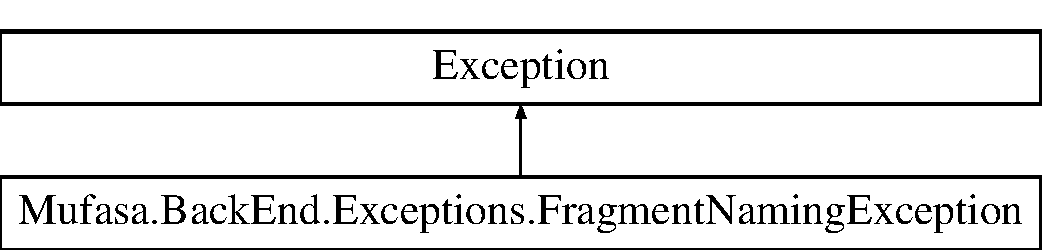
\includegraphics[height=2.000000cm]{class_mufasa_1_1_back_end_1_1_exceptions_1_1_fragment_naming_exception}
\end{center}
\end{figure}
\subsection*{Public Member Functions}
\begin{DoxyCompactItemize}
\item 
\hyperlink{class_mufasa_1_1_back_end_1_1_exceptions_1_1_fragment_naming_exception_a8c1ca1a4f964e73a9da693808f33d386}{Fragment\+Naming\+Exception} ()
\begin{DoxyCompactList}\small\item\em \hyperlink{class_mufasa_1_1_back_end_1_1_exceptions_1_1_fragment_naming_exception}{Fragment\+Naming\+Exception} constructor. \end{DoxyCompactList}\item 
\hyperlink{class_mufasa_1_1_back_end_1_1_exceptions_1_1_fragment_naming_exception_aaa478e87d5cfe6831f0adf4aa5af0cec}{Fragment\+Naming\+Exception} (string message)
\begin{DoxyCompactList}\small\item\em \hyperlink{class_mufasa_1_1_back_end_1_1_exceptions_1_1_fragment_naming_exception}{Fragment\+Naming\+Exception} constructor. \end{DoxyCompactList}\end{DoxyCompactItemize}


\subsection{Detailed Description}
Exception thrown if a fragment name is invalid. Back\+End.\+Designer.\+Designer.\+cs 

Definition at line 13 of file Fragment\+Naming\+Exception.\+cs.



\subsection{Constructor \& Destructor Documentation}
\hypertarget{class_mufasa_1_1_back_end_1_1_exceptions_1_1_fragment_naming_exception_a8c1ca1a4f964e73a9da693808f33d386}{\index{Mufasa\+::\+Back\+End\+::\+Exceptions\+::\+Fragment\+Naming\+Exception@{Mufasa\+::\+Back\+End\+::\+Exceptions\+::\+Fragment\+Naming\+Exception}!Fragment\+Naming\+Exception@{Fragment\+Naming\+Exception}}
\index{Fragment\+Naming\+Exception@{Fragment\+Naming\+Exception}!Mufasa\+::\+Back\+End\+::\+Exceptions\+::\+Fragment\+Naming\+Exception@{Mufasa\+::\+Back\+End\+::\+Exceptions\+::\+Fragment\+Naming\+Exception}}
\subsubsection[{Fragment\+Naming\+Exception}]{\setlength{\rightskip}{0pt plus 5cm}Mufasa.\+Back\+End.\+Exceptions.\+Fragment\+Naming\+Exception.\+Fragment\+Naming\+Exception (
\begin{DoxyParamCaption}
{}
\end{DoxyParamCaption}
)}}\label{class_mufasa_1_1_back_end_1_1_exceptions_1_1_fragment_naming_exception_a8c1ca1a4f964e73a9da693808f33d386}


\hyperlink{class_mufasa_1_1_back_end_1_1_exceptions_1_1_fragment_naming_exception}{Fragment\+Naming\+Exception} constructor. 



Definition at line 18 of file Fragment\+Naming\+Exception.\+cs.

\hypertarget{class_mufasa_1_1_back_end_1_1_exceptions_1_1_fragment_naming_exception_aaa478e87d5cfe6831f0adf4aa5af0cec}{\index{Mufasa\+::\+Back\+End\+::\+Exceptions\+::\+Fragment\+Naming\+Exception@{Mufasa\+::\+Back\+End\+::\+Exceptions\+::\+Fragment\+Naming\+Exception}!Fragment\+Naming\+Exception@{Fragment\+Naming\+Exception}}
\index{Fragment\+Naming\+Exception@{Fragment\+Naming\+Exception}!Mufasa\+::\+Back\+End\+::\+Exceptions\+::\+Fragment\+Naming\+Exception@{Mufasa\+::\+Back\+End\+::\+Exceptions\+::\+Fragment\+Naming\+Exception}}
\subsubsection[{Fragment\+Naming\+Exception}]{\setlength{\rightskip}{0pt plus 5cm}Mufasa.\+Back\+End.\+Exceptions.\+Fragment\+Naming\+Exception.\+Fragment\+Naming\+Exception (
\begin{DoxyParamCaption}
\item[{string}]{message}
\end{DoxyParamCaption}
)}}\label{class_mufasa_1_1_back_end_1_1_exceptions_1_1_fragment_naming_exception_aaa478e87d5cfe6831f0adf4aa5af0cec}


\hyperlink{class_mufasa_1_1_back_end_1_1_exceptions_1_1_fragment_naming_exception}{Fragment\+Naming\+Exception} constructor. 


\begin{DoxyParams}{Parameters}
{\em message} & Message to send.\\
\hline
\end{DoxyParams}


Definition at line 27 of file Fragment\+Naming\+Exception.\+cs.



The documentation for this class was generated from the following file\+:\begin{DoxyCompactItemize}
\item 
Mufasa/\+Mufasa/\+Back\+End/\+Exceptions/\hyperlink{_fragment_naming_exception_8cs}{Fragment\+Naming\+Exception.\+cs}\end{DoxyCompactItemize}

\hypertarget{class_mufasa_1_1_main_window}{\section{Mufasa.\+Main\+Window Class Reference}
\label{class_mufasa_1_1_main_window}\index{Mufasa.\+Main\+Window@{Mufasa.\+Main\+Window}}
}


Interaction logic for Main\+Window.\+xaml  


Inheritance diagram for Mufasa.\+Main\+Window\+:\begin{figure}[H]
\begin{center}
\leavevmode
\includegraphics[height=1.544828cm]{class_mufasa_1_1_main_window}
\end{center}
\end{figure}
\subsection*{Public Member Functions}
\begin{DoxyCompactItemize}
\item 
\hyperlink{class_mufasa_1_1_main_window_afea7727fa66912c6a590a0a631de1586}{Main\+Window} ()
\item 
void \hyperlink{class_mufasa_1_1_main_window_aa80bd3c2337c0a5d6e25fab789f54734}{Initialize\+Component} ()
\begin{DoxyCompactList}\small\item\em Initialize\+Component \end{DoxyCompactList}\item 
void \hyperlink{class_mufasa_1_1_main_window_aa80bd3c2337c0a5d6e25fab789f54734}{Initialize\+Component} ()
\begin{DoxyCompactList}\small\item\em Initialize\+Component \end{DoxyCompactList}\end{DoxyCompactItemize}


\subsection{Detailed Description}
Interaction logic for Main\+Window.\+xaml 

\hyperlink{class_mufasa_1_1_main_window}{Main\+Window} 

Definition at line 22 of file Main\+Window.\+xaml.\+cs.



\subsection{Constructor \& Destructor Documentation}
\hypertarget{class_mufasa_1_1_main_window_afea7727fa66912c6a590a0a631de1586}{\index{Mufasa\+::\+Main\+Window@{Mufasa\+::\+Main\+Window}!Main\+Window@{Main\+Window}}
\index{Main\+Window@{Main\+Window}!Mufasa\+::\+Main\+Window@{Mufasa\+::\+Main\+Window}}
\subsubsection[{Main\+Window}]{\setlength{\rightskip}{0pt plus 5cm}Mufasa.\+Main\+Window.\+Main\+Window (
\begin{DoxyParamCaption}
{}
\end{DoxyParamCaption}
)}}\label{class_mufasa_1_1_main_window_afea7727fa66912c6a590a0a631de1586}


Definition at line 24 of file Main\+Window.\+xaml.\+cs.



\subsection{Member Function Documentation}
\hypertarget{class_mufasa_1_1_main_window_aa80bd3c2337c0a5d6e25fab789f54734}{\index{Mufasa\+::\+Main\+Window@{Mufasa\+::\+Main\+Window}!Initialize\+Component@{Initialize\+Component}}
\index{Initialize\+Component@{Initialize\+Component}!Mufasa\+::\+Main\+Window@{Mufasa\+::\+Main\+Window}}
\subsubsection[{Initialize\+Component}]{\setlength{\rightskip}{0pt plus 5cm}void Mufasa.\+Main\+Window.\+Initialize\+Component (
\begin{DoxyParamCaption}
{}
\end{DoxyParamCaption}
)}}\label{class_mufasa_1_1_main_window_aa80bd3c2337c0a5d6e25fab789f54734}


Initialize\+Component 



Definition at line 54 of file Main\+Window.\+g.\+cs.

\hypertarget{class_mufasa_1_1_main_window_aa80bd3c2337c0a5d6e25fab789f54734}{\index{Mufasa\+::\+Main\+Window@{Mufasa\+::\+Main\+Window}!Initialize\+Component@{Initialize\+Component}}
\index{Initialize\+Component@{Initialize\+Component}!Mufasa\+::\+Main\+Window@{Mufasa\+::\+Main\+Window}}
\subsubsection[{Initialize\+Component}]{\setlength{\rightskip}{0pt plus 5cm}void Mufasa.\+Main\+Window.\+Initialize\+Component (
\begin{DoxyParamCaption}
{}
\end{DoxyParamCaption}
)}}\label{class_mufasa_1_1_main_window_aa80bd3c2337c0a5d6e25fab789f54734}


Initialize\+Component 



Definition at line 54 of file Main\+Window.\+g.\+i.\+cs.



The documentation for this class was generated from the following files\+:\begin{DoxyCompactItemize}
\item 
Mufasa/\+Mufasa/\hyperlink{_main_window_8xaml_8cs}{Main\+Window.\+xaml.\+cs}\item 
Mufasa/\+Mufasa/obj/\+Debug/\hyperlink{_main_window_8g_8cs}{Main\+Window.\+g.\+cs}\item 
Mufasa/\+Mufasa/obj/\+Debug/\hyperlink{_main_window_8g_8i_8cs}{Main\+Window.\+g.\+i.\+cs}\end{DoxyCompactItemize}

\hypertarget{class_mufasa_1_1_pages_1_1_reaction}{\section{Mufasa.\+Pages.\+Reaction Class Reference}
\label{class_mufasa_1_1_pages_1_1_reaction}\index{Mufasa.\+Pages.\+Reaction@{Mufasa.\+Pages.\+Reaction}}
}


\hyperlink{class_mufasa_1_1_pages_1_1_reaction}{Reaction}  


Inheritance diagram for Mufasa.\+Pages.\+Reaction\+:\begin{figure}[H]
\begin{center}
\leavevmode
\includegraphics[height=1.454545cm]{class_mufasa_1_1_pages_1_1_reaction}
\end{center}
\end{figure}
\subsection*{Public Member Functions}
\begin{DoxyCompactItemize}
\item 
void \hyperlink{class_mufasa_1_1_pages_1_1_reaction_a0203f4fc272b7da8e61646e337ad270b}{Initialize\+Component} ()
\begin{DoxyCompactList}\small\item\em Initialize\+Component \end{DoxyCompactList}\item 
void \hyperlink{class_mufasa_1_1_pages_1_1_reaction_a0203f4fc272b7da8e61646e337ad270b}{Initialize\+Component} ()
\begin{DoxyCompactList}\small\item\em Initialize\+Component \end{DoxyCompactList}\item 
\hyperlink{class_mufasa_1_1_pages_1_1_reaction_ae7656aa4b7df6b27160d230b705a5763}{Reaction} ()
\end{DoxyCompactItemize}


\subsection{Detailed Description}
\hyperlink{class_mufasa_1_1_pages_1_1_reaction}{Reaction} 

Interaction logic for Reaction.\+xaml 

Definition at line 45 of file Reaction.\+g.\+cs.



\subsection{Constructor \& Destructor Documentation}
\hypertarget{class_mufasa_1_1_pages_1_1_reaction_ae7656aa4b7df6b27160d230b705a5763}{\index{Mufasa\+::\+Pages\+::\+Reaction@{Mufasa\+::\+Pages\+::\+Reaction}!Reaction@{Reaction}}
\index{Reaction@{Reaction}!Mufasa\+::\+Pages\+::\+Reaction@{Mufasa\+::\+Pages\+::\+Reaction}}
\subsubsection[{Reaction}]{\setlength{\rightskip}{0pt plus 5cm}Mufasa.\+Pages.\+Reaction.\+Reaction (
\begin{DoxyParamCaption}
{}
\end{DoxyParamCaption}
)}}\label{class_mufasa_1_1_pages_1_1_reaction_ae7656aa4b7df6b27160d230b705a5763}


Definition at line 23 of file Reaction.\+xaml.\+cs.



\subsection{Member Function Documentation}
\hypertarget{class_mufasa_1_1_pages_1_1_reaction_a0203f4fc272b7da8e61646e337ad270b}{\index{Mufasa\+::\+Pages\+::\+Reaction@{Mufasa\+::\+Pages\+::\+Reaction}!Initialize\+Component@{Initialize\+Component}}
\index{Initialize\+Component@{Initialize\+Component}!Mufasa\+::\+Pages\+::\+Reaction@{Mufasa\+::\+Pages\+::\+Reaction}}
\subsubsection[{Initialize\+Component}]{\setlength{\rightskip}{0pt plus 5cm}void Mufasa.\+Pages.\+Reaction.\+Initialize\+Component (
\begin{DoxyParamCaption}
{}
\end{DoxyParamCaption}
)}}\label{class_mufasa_1_1_pages_1_1_reaction_a0203f4fc272b7da8e61646e337ad270b}


Initialize\+Component 



Definition at line 54 of file Reaction.\+g.\+cs.

\hypertarget{class_mufasa_1_1_pages_1_1_reaction_a0203f4fc272b7da8e61646e337ad270b}{\index{Mufasa\+::\+Pages\+::\+Reaction@{Mufasa\+::\+Pages\+::\+Reaction}!Initialize\+Component@{Initialize\+Component}}
\index{Initialize\+Component@{Initialize\+Component}!Mufasa\+::\+Pages\+::\+Reaction@{Mufasa\+::\+Pages\+::\+Reaction}}
\subsubsection[{Initialize\+Component}]{\setlength{\rightskip}{0pt plus 5cm}void Mufasa.\+Pages.\+Reaction.\+Initialize\+Component (
\begin{DoxyParamCaption}
{}
\end{DoxyParamCaption}
)}}\label{class_mufasa_1_1_pages_1_1_reaction_a0203f4fc272b7da8e61646e337ad270b}


Initialize\+Component 



Definition at line 54 of file Reaction.\+g.\+i.\+cs.



The documentation for this class was generated from the following files\+:\begin{DoxyCompactItemize}
\item 
Mufasa/\+Mufasa/obj/\+Debug/\+Pages/\hyperlink{_reaction_8g_8cs}{Reaction.\+g.\+cs}\item 
Mufasa/\+Mufasa/obj/\+Debug/\+Pages/\hyperlink{_reaction_8g_8i_8cs}{Reaction.\+g.\+i.\+cs}\item 
Mufasa/\+Mufasa/\+Pages/\hyperlink{_reaction_8xaml_8cs}{Reaction.\+xaml.\+cs}\end{DoxyCompactItemize}

\hypertarget{class_mufasa_1_1_back_end_1_1_exceptions_1_1_sequence_count_exception}{\section{Mufasa.\+Back\+End.\+Exceptions.\+Sequence\+Count\+Exception Class Reference}
\label{class_mufasa_1_1_back_end_1_1_exceptions_1_1_sequence_count_exception}\index{Mufasa.\+Back\+End.\+Exceptions.\+Sequence\+Count\+Exception@{Mufasa.\+Back\+End.\+Exceptions.\+Sequence\+Count\+Exception}}
}
Inheritance diagram for Mufasa.\+Back\+End.\+Exceptions.\+Sequence\+Count\+Exception\+:\begin{figure}[H]
\begin{center}
\leavevmode
\includegraphics[height=2.000000cm]{class_mufasa_1_1_back_end_1_1_exceptions_1_1_sequence_count_exception}
\end{center}
\end{figure}
\subsection*{Public Member Functions}
\begin{DoxyCompactItemize}
\item 
\hyperlink{class_mufasa_1_1_back_end_1_1_exceptions_1_1_sequence_count_exception_a7145b5fb8b3ab93b145e583bcc813c32}{Sequence\+Count\+Exception} ()
\begin{DoxyCompactList}\small\item\em \hyperlink{class_mufasa_1_1_back_end_1_1_exceptions_1_1_sequence_count_exception}{Sequence\+Count\+Exception} constructor. \end{DoxyCompactList}\item 
\hyperlink{class_mufasa_1_1_back_end_1_1_exceptions_1_1_sequence_count_exception_a4a24df40384bb9e496adba815496bb80}{Sequence\+Count\+Exception} (string message)
\begin{DoxyCompactList}\small\item\em \hyperlink{class_mufasa_1_1_back_end_1_1_exceptions_1_1_sequence_count_exception}{Sequence\+Count\+Exception} constructor. \end{DoxyCompactList}\end{DoxyCompactItemize}


\subsection{Detailed Description}
Exception thrown if sequence count in a file is invalid. Back\+End.\+Designer.\+Designer.\+cs 

Definition at line 13 of file Sequence\+Count\+Exception.\+cs.



\subsection{Constructor \& Destructor Documentation}
\hypertarget{class_mufasa_1_1_back_end_1_1_exceptions_1_1_sequence_count_exception_a7145b5fb8b3ab93b145e583bcc813c32}{\index{Mufasa\+::\+Back\+End\+::\+Exceptions\+::\+Sequence\+Count\+Exception@{Mufasa\+::\+Back\+End\+::\+Exceptions\+::\+Sequence\+Count\+Exception}!Sequence\+Count\+Exception@{Sequence\+Count\+Exception}}
\index{Sequence\+Count\+Exception@{Sequence\+Count\+Exception}!Mufasa\+::\+Back\+End\+::\+Exceptions\+::\+Sequence\+Count\+Exception@{Mufasa\+::\+Back\+End\+::\+Exceptions\+::\+Sequence\+Count\+Exception}}
\subsubsection[{Sequence\+Count\+Exception}]{\setlength{\rightskip}{0pt plus 5cm}Mufasa.\+Back\+End.\+Exceptions.\+Sequence\+Count\+Exception.\+Sequence\+Count\+Exception (
\begin{DoxyParamCaption}
{}
\end{DoxyParamCaption}
)}}\label{class_mufasa_1_1_back_end_1_1_exceptions_1_1_sequence_count_exception_a7145b5fb8b3ab93b145e583bcc813c32}


\hyperlink{class_mufasa_1_1_back_end_1_1_exceptions_1_1_sequence_count_exception}{Sequence\+Count\+Exception} constructor. 



Definition at line 18 of file Sequence\+Count\+Exception.\+cs.

\hypertarget{class_mufasa_1_1_back_end_1_1_exceptions_1_1_sequence_count_exception_a4a24df40384bb9e496adba815496bb80}{\index{Mufasa\+::\+Back\+End\+::\+Exceptions\+::\+Sequence\+Count\+Exception@{Mufasa\+::\+Back\+End\+::\+Exceptions\+::\+Sequence\+Count\+Exception}!Sequence\+Count\+Exception@{Sequence\+Count\+Exception}}
\index{Sequence\+Count\+Exception@{Sequence\+Count\+Exception}!Mufasa\+::\+Back\+End\+::\+Exceptions\+::\+Sequence\+Count\+Exception@{Mufasa\+::\+Back\+End\+::\+Exceptions\+::\+Sequence\+Count\+Exception}}
\subsubsection[{Sequence\+Count\+Exception}]{\setlength{\rightskip}{0pt plus 5cm}Mufasa.\+Back\+End.\+Exceptions.\+Sequence\+Count\+Exception.\+Sequence\+Count\+Exception (
\begin{DoxyParamCaption}
\item[{string}]{message}
\end{DoxyParamCaption}
)}}\label{class_mufasa_1_1_back_end_1_1_exceptions_1_1_sequence_count_exception_a4a24df40384bb9e496adba815496bb80}


\hyperlink{class_mufasa_1_1_back_end_1_1_exceptions_1_1_sequence_count_exception}{Sequence\+Count\+Exception} constructor. 


\begin{DoxyParams}{Parameters}
{\em message} & Message to send.\\
\hline
\end{DoxyParams}


Definition at line 27 of file Sequence\+Count\+Exception.\+cs.



The documentation for this class was generated from the following file\+:\begin{DoxyCompactItemize}
\item 
Mufasa/\+Mufasa/\+Back\+End/\+Exceptions/\hyperlink{_sequence_count_exception_8cs}{Sequence\+Count\+Exception.\+cs}\end{DoxyCompactItemize}

\hypertarget{class_mufasa_1_1_back_end_1_1_exceptions_1_1_sequence_length_exception}{\section{Mufasa.\+Back\+End.\+Exceptions.\+Sequence\+Length\+Exception Class Reference}
\label{class_mufasa_1_1_back_end_1_1_exceptions_1_1_sequence_length_exception}\index{Mufasa.\+Back\+End.\+Exceptions.\+Sequence\+Length\+Exception@{Mufasa.\+Back\+End.\+Exceptions.\+Sequence\+Length\+Exception}}
}
Inheritance diagram for Mufasa.\+Back\+End.\+Exceptions.\+Sequence\+Length\+Exception\+:\begin{figure}[H]
\begin{center}
\leavevmode
\includegraphics[height=2.000000cm]{class_mufasa_1_1_back_end_1_1_exceptions_1_1_sequence_length_exception}
\end{center}
\end{figure}
\subsection*{Public Member Functions}
\begin{DoxyCompactItemize}
\item 
\hyperlink{class_mufasa_1_1_back_end_1_1_exceptions_1_1_sequence_length_exception_a8e6429f888d625777a07b62f076e2ff7}{Sequence\+Length\+Exception} ()
\begin{DoxyCompactList}\small\item\em \hyperlink{class_mufasa_1_1_back_end_1_1_exceptions_1_1_sequence_length_exception}{Sequence\+Length\+Exception} constructor. \end{DoxyCompactList}\item 
\hyperlink{class_mufasa_1_1_back_end_1_1_exceptions_1_1_sequence_length_exception_a93a95c1b7f6d0214128bea0935ebf8c2}{Sequence\+Length\+Exception} (string message)
\begin{DoxyCompactList}\small\item\em \hyperlink{class_mufasa_1_1_back_end_1_1_exceptions_1_1_sequence_length_exception}{Sequence\+Length\+Exception} constructor. \end{DoxyCompactList}\item 
\hyperlink{class_mufasa_1_1_back_end_1_1_exceptions_1_1_sequence_length_exception_ab69a9738667e974436ffe38e2f038aef}{Sequence\+Length\+Exception} (string message, I\+Sequence sequence)
\begin{DoxyCompactList}\small\item\em \hyperlink{class_mufasa_1_1_back_end_1_1_exceptions_1_1_sequence_length_exception}{Sequence\+Length\+Exception} constructor. \end{DoxyCompactList}\end{DoxyCompactItemize}
\subsection*{Properties}
\begin{DoxyCompactItemize}
\item 
I\+Sequence \hyperlink{class_mufasa_1_1_back_end_1_1_exceptions_1_1_sequence_length_exception_ace577fe27718b807b7468270750aef00}{Sequence}\hspace{0.3cm}{\ttfamily  \mbox{[}get, set\mbox{]}}
\begin{DoxyCompactList}\small\item\em Sequence in question. \end{DoxyCompactList}\end{DoxyCompactItemize}


\subsection{Detailed Description}
Exception thrown if sequence length in a file is invalid. Back\+End.\+Designer.\+Designer.\+cs 

Definition at line 14 of file Sequence\+Length\+Exception.\+cs.



\subsection{Constructor \& Destructor Documentation}
\hypertarget{class_mufasa_1_1_back_end_1_1_exceptions_1_1_sequence_length_exception_a8e6429f888d625777a07b62f076e2ff7}{\index{Mufasa\+::\+Back\+End\+::\+Exceptions\+::\+Sequence\+Length\+Exception@{Mufasa\+::\+Back\+End\+::\+Exceptions\+::\+Sequence\+Length\+Exception}!Sequence\+Length\+Exception@{Sequence\+Length\+Exception}}
\index{Sequence\+Length\+Exception@{Sequence\+Length\+Exception}!Mufasa\+::\+Back\+End\+::\+Exceptions\+::\+Sequence\+Length\+Exception@{Mufasa\+::\+Back\+End\+::\+Exceptions\+::\+Sequence\+Length\+Exception}}
\subsubsection[{Sequence\+Length\+Exception}]{\setlength{\rightskip}{0pt plus 5cm}Mufasa.\+Back\+End.\+Exceptions.\+Sequence\+Length\+Exception.\+Sequence\+Length\+Exception (
\begin{DoxyParamCaption}
{}
\end{DoxyParamCaption}
)}}\label{class_mufasa_1_1_back_end_1_1_exceptions_1_1_sequence_length_exception_a8e6429f888d625777a07b62f076e2ff7}


\hyperlink{class_mufasa_1_1_back_end_1_1_exceptions_1_1_sequence_length_exception}{Sequence\+Length\+Exception} constructor. 



Definition at line 24 of file Sequence\+Length\+Exception.\+cs.

\hypertarget{class_mufasa_1_1_back_end_1_1_exceptions_1_1_sequence_length_exception_a93a95c1b7f6d0214128bea0935ebf8c2}{\index{Mufasa\+::\+Back\+End\+::\+Exceptions\+::\+Sequence\+Length\+Exception@{Mufasa\+::\+Back\+End\+::\+Exceptions\+::\+Sequence\+Length\+Exception}!Sequence\+Length\+Exception@{Sequence\+Length\+Exception}}
\index{Sequence\+Length\+Exception@{Sequence\+Length\+Exception}!Mufasa\+::\+Back\+End\+::\+Exceptions\+::\+Sequence\+Length\+Exception@{Mufasa\+::\+Back\+End\+::\+Exceptions\+::\+Sequence\+Length\+Exception}}
\subsubsection[{Sequence\+Length\+Exception}]{\setlength{\rightskip}{0pt plus 5cm}Mufasa.\+Back\+End.\+Exceptions.\+Sequence\+Length\+Exception.\+Sequence\+Length\+Exception (
\begin{DoxyParamCaption}
\item[{string}]{message}
\end{DoxyParamCaption}
)}}\label{class_mufasa_1_1_back_end_1_1_exceptions_1_1_sequence_length_exception_a93a95c1b7f6d0214128bea0935ebf8c2}


\hyperlink{class_mufasa_1_1_back_end_1_1_exceptions_1_1_sequence_length_exception}{Sequence\+Length\+Exception} constructor. 


\begin{DoxyParams}{Parameters}
{\em message} & Message to send.\\
\hline
\end{DoxyParams}


Definition at line 34 of file Sequence\+Length\+Exception.\+cs.

\hypertarget{class_mufasa_1_1_back_end_1_1_exceptions_1_1_sequence_length_exception_ab69a9738667e974436ffe38e2f038aef}{\index{Mufasa\+::\+Back\+End\+::\+Exceptions\+::\+Sequence\+Length\+Exception@{Mufasa\+::\+Back\+End\+::\+Exceptions\+::\+Sequence\+Length\+Exception}!Sequence\+Length\+Exception@{Sequence\+Length\+Exception}}
\index{Sequence\+Length\+Exception@{Sequence\+Length\+Exception}!Mufasa\+::\+Back\+End\+::\+Exceptions\+::\+Sequence\+Length\+Exception@{Mufasa\+::\+Back\+End\+::\+Exceptions\+::\+Sequence\+Length\+Exception}}
\subsubsection[{Sequence\+Length\+Exception}]{\setlength{\rightskip}{0pt plus 5cm}Mufasa.\+Back\+End.\+Exceptions.\+Sequence\+Length\+Exception.\+Sequence\+Length\+Exception (
\begin{DoxyParamCaption}
\item[{string}]{message, }
\item[{I\+Sequence}]{sequence}
\end{DoxyParamCaption}
)}}\label{class_mufasa_1_1_back_end_1_1_exceptions_1_1_sequence_length_exception_ab69a9738667e974436ffe38e2f038aef}


\hyperlink{class_mufasa_1_1_back_end_1_1_exceptions_1_1_sequence_length_exception}{Sequence\+Length\+Exception} constructor. 


\begin{DoxyParams}{Parameters}
{\em message} & Message to send.\\
\hline
{\em sequence} & Sequence in question.\\
\hline
\end{DoxyParams}


Definition at line 45 of file Sequence\+Length\+Exception.\+cs.



\subsection{Property Documentation}
\hypertarget{class_mufasa_1_1_back_end_1_1_exceptions_1_1_sequence_length_exception_ace577fe27718b807b7468270750aef00}{\index{Mufasa\+::\+Back\+End\+::\+Exceptions\+::\+Sequence\+Length\+Exception@{Mufasa\+::\+Back\+End\+::\+Exceptions\+::\+Sequence\+Length\+Exception}!Sequence@{Sequence}}
\index{Sequence@{Sequence}!Mufasa\+::\+Back\+End\+::\+Exceptions\+::\+Sequence\+Length\+Exception@{Mufasa\+::\+Back\+End\+::\+Exceptions\+::\+Sequence\+Length\+Exception}}
\subsubsection[{Sequence}]{\setlength{\rightskip}{0pt plus 5cm}I\+Sequence Mufasa.\+Back\+End.\+Exceptions.\+Sequence\+Length\+Exception.\+Sequence\hspace{0.3cm}{\ttfamily [get]}, {\ttfamily [set]}}}\label{class_mufasa_1_1_back_end_1_1_exceptions_1_1_sequence_length_exception_ace577fe27718b807b7468270750aef00}


Sequence in question. 



Definition at line 19 of file Sequence\+Length\+Exception.\+cs.



The documentation for this class was generated from the following file\+:\begin{DoxyCompactItemize}
\item 
Mufasa/\+Mufasa/\+Back\+End/\+Exceptions/\hyperlink{_sequence_length_exception_8cs}{Sequence\+Length\+Exception.\+cs}\end{DoxyCompactItemize}

\hypertarget{class_mufasa_1_1_pages_1_1_settings_page}{\section{Mufasa.\+Pages.\+Settings\+Page Class Reference}
\label{class_mufasa_1_1_pages_1_1_settings_page}\index{Mufasa.\+Pages.\+Settings\+Page@{Mufasa.\+Pages.\+Settings\+Page}}
}


\hyperlink{class_mufasa_1_1_pages_1_1_settings_page}{Settings\+Page}  


Inheritance diagram for Mufasa.\+Pages.\+Settings\+Page\+:\begin{figure}[H]
\begin{center}
\leavevmode
\includegraphics[height=1.258427cm]{class_mufasa_1_1_pages_1_1_settings_page}
\end{center}
\end{figure}
\subsection*{Public Member Functions}
\begin{DoxyCompactItemize}
\item 
void \hyperlink{class_mufasa_1_1_pages_1_1_settings_page_a32052ee7f930dd459c8e572d38a97b1c}{Initialize\+Component} ()
\begin{DoxyCompactList}\small\item\em Initialize\+Component \end{DoxyCompactList}\item 
void \hyperlink{class_mufasa_1_1_pages_1_1_settings_page_a32052ee7f930dd459c8e572d38a97b1c}{Initialize\+Component} ()
\begin{DoxyCompactList}\small\item\em Initialize\+Component \end{DoxyCompactList}\item 
\hyperlink{class_mufasa_1_1_pages_1_1_settings_page_a8fdb70faa36c8d90b0b97a3fd8d9667b}{Settings\+Page} ()
\end{DoxyCompactItemize}


\subsection{Detailed Description}
\hyperlink{class_mufasa_1_1_pages_1_1_settings_page}{Settings\+Page} 

Interaction logic for Settings\+Page.\+xaml 

Definition at line 45 of file Settings\+Page.\+g.\+cs.



\subsection{Constructor \& Destructor Documentation}
\hypertarget{class_mufasa_1_1_pages_1_1_settings_page_a8fdb70faa36c8d90b0b97a3fd8d9667b}{\index{Mufasa\+::\+Pages\+::\+Settings\+Page@{Mufasa\+::\+Pages\+::\+Settings\+Page}!Settings\+Page@{Settings\+Page}}
\index{Settings\+Page@{Settings\+Page}!Mufasa\+::\+Pages\+::\+Settings\+Page@{Mufasa\+::\+Pages\+::\+Settings\+Page}}
\subsubsection[{Settings\+Page}]{\setlength{\rightskip}{0pt plus 5cm}Mufasa.\+Pages.\+Settings\+Page.\+Settings\+Page (
\begin{DoxyParamCaption}
{}
\end{DoxyParamCaption}
)}}\label{class_mufasa_1_1_pages_1_1_settings_page_a8fdb70faa36c8d90b0b97a3fd8d9667b}


Definition at line 23 of file Settings\+Page.\+xaml.\+cs.



\subsection{Member Function Documentation}
\hypertarget{class_mufasa_1_1_pages_1_1_settings_page_a32052ee7f930dd459c8e572d38a97b1c}{\index{Mufasa\+::\+Pages\+::\+Settings\+Page@{Mufasa\+::\+Pages\+::\+Settings\+Page}!Initialize\+Component@{Initialize\+Component}}
\index{Initialize\+Component@{Initialize\+Component}!Mufasa\+::\+Pages\+::\+Settings\+Page@{Mufasa\+::\+Pages\+::\+Settings\+Page}}
\subsubsection[{Initialize\+Component}]{\setlength{\rightskip}{0pt plus 5cm}void Mufasa.\+Pages.\+Settings\+Page.\+Initialize\+Component (
\begin{DoxyParamCaption}
{}
\end{DoxyParamCaption}
)}}\label{class_mufasa_1_1_pages_1_1_settings_page_a32052ee7f930dd459c8e572d38a97b1c}


Initialize\+Component 



Definition at line 54 of file Settings\+Page.\+g.\+cs.

\hypertarget{class_mufasa_1_1_pages_1_1_settings_page_a32052ee7f930dd459c8e572d38a97b1c}{\index{Mufasa\+::\+Pages\+::\+Settings\+Page@{Mufasa\+::\+Pages\+::\+Settings\+Page}!Initialize\+Component@{Initialize\+Component}}
\index{Initialize\+Component@{Initialize\+Component}!Mufasa\+::\+Pages\+::\+Settings\+Page@{Mufasa\+::\+Pages\+::\+Settings\+Page}}
\subsubsection[{Initialize\+Component}]{\setlength{\rightskip}{0pt plus 5cm}void Mufasa.\+Pages.\+Settings\+Page.\+Initialize\+Component (
\begin{DoxyParamCaption}
{}
\end{DoxyParamCaption}
)}}\label{class_mufasa_1_1_pages_1_1_settings_page_a32052ee7f930dd459c8e572d38a97b1c}


Initialize\+Component 



Definition at line 54 of file Settings\+Page.\+g.\+i.\+cs.



The documentation for this class was generated from the following files\+:\begin{DoxyCompactItemize}
\item 
Mufasa/\+Mufasa/obj/\+Debug/\+Pages/\hyperlink{_settings_page_8g_8cs}{Settings\+Page.\+g.\+cs}\item 
Mufasa/\+Mufasa/obj/\+Debug/\+Pages/\hyperlink{_settings_page_8g_8i_8cs}{Settings\+Page.\+g.\+i.\+cs}\item 
Mufasa/\+Mufasa/\+Pages/\hyperlink{_settings_page_8xaml_8cs}{Settings\+Page.\+xaml.\+cs}\end{DoxyCompactItemize}

\chapter{File Documentation}
\hypertarget{_app_8xaml_8cs}{\section{Mufasa/\+Mufasa/\+App.xaml.\+cs File Reference}
\label{_app_8xaml_8cs}\index{Mufasa/\+Mufasa/\+App.\+xaml.\+cs@{Mufasa/\+Mufasa/\+App.\+xaml.\+cs}}
}
\subsection*{Classes}
\begin{DoxyCompactItemize}
\item 
class \hyperlink{class_mufasa_1_1_app}{Mufasa.\+App}
\begin{DoxyCompactList}\small\item\em Interaction logic for App.\+xaml \end{DoxyCompactList}\end{DoxyCompactItemize}
\subsection*{Namespaces}
\begin{DoxyCompactItemize}
\item 
package \hyperlink{namespace_mufasa}{Mufasa}
\end{DoxyCompactItemize}

\hypertarget{_construct_8cs}{\section{Mufasa/\+Mufasa/\+Back\+End/\+Designer/\+Construct.cs File Reference}
\label{_construct_8cs}\index{Mufasa/\+Mufasa/\+Back\+End/\+Designer/\+Construct.\+cs@{Mufasa/\+Mufasa/\+Back\+End/\+Designer/\+Construct.\+cs}}
}
\subsection*{Classes}
\begin{DoxyCompactItemize}
\item 
class \hyperlink{class_mufasa_1_1_back_end_1_1_designer_1_1_construct}{Mufasa.\+Back\+End.\+Designer.\+Construct}
\end{DoxyCompactItemize}
\subsection*{Namespaces}
\begin{DoxyCompactItemize}
\item 
package \hyperlink{namespace_mufasa_1_1_back_end_1_1_designer}{Mufasa.\+Back\+End.\+Designer}
\end{DoxyCompactItemize}

\hypertarget{_designer_8cs}{\section{Mufasa/\+Mufasa/\+Back\+End/\+Designer/\+Designer.cs File Reference}
\label{_designer_8cs}\index{Mufasa/\+Mufasa/\+Back\+End/\+Designer/\+Designer.\+cs@{Mufasa/\+Mufasa/\+Back\+End/\+Designer/\+Designer.\+cs}}
}
\subsection*{Classes}
\begin{DoxyCompactItemize}
\item 
class \hyperlink{class_mufasa_1_1_back_end_1_1_designer_1_1_designer}{Mufasa.\+Back\+End.\+Designer.\+Designer}
\end{DoxyCompactItemize}
\subsection*{Namespaces}
\begin{DoxyCompactItemize}
\item 
package \hyperlink{namespace_mufasa_1_1_back_end_1_1_designer}{Mufasa.\+Back\+End.\+Designer}
\end{DoxyCompactItemize}

\hypertarget{_fragment_8cs}{\section{Mufasa/\+Mufasa/\+Back\+End/\+Designer/\+Fragment.cs File Reference}
\label{_fragment_8cs}\index{Mufasa/\+Mufasa/\+Back\+End/\+Designer/\+Fragment.\+cs@{Mufasa/\+Mufasa/\+Back\+End/\+Designer/\+Fragment.\+cs}}
}
\subsection*{Classes}
\begin{DoxyCompactItemize}
\item 
class \hyperlink{class_mufasa_1_1_back_end_1_1_designer_1_1_fragment}{Mufasa.\+Back\+End.\+Designer.\+Fragment}
\end{DoxyCompactItemize}
\subsection*{Namespaces}
\begin{DoxyCompactItemize}
\item 
package \hyperlink{namespace_mufasa_1_1_back_end_1_1_designer}{Mufasa.\+Back\+End.\+Designer}
\end{DoxyCompactItemize}

\input{_fragment_naming_exception_8cs}
\hypertarget{_sequence_count_exception_8cs}{\section{Mufasa/\+Mufasa/\+Back\+End/\+Exceptions/\+Sequence\+Count\+Exception.cs File Reference}
\label{_sequence_count_exception_8cs}\index{Mufasa/\+Mufasa/\+Back\+End/\+Exceptions/\+Sequence\+Count\+Exception.\+cs@{Mufasa/\+Mufasa/\+Back\+End/\+Exceptions/\+Sequence\+Count\+Exception.\+cs}}
}
\subsection*{Classes}
\begin{DoxyCompactItemize}
\item 
class \hyperlink{class_mufasa_1_1_back_end_1_1_exceptions_1_1_sequence_count_exception}{Mufasa.\+Back\+End.\+Exceptions.\+Sequence\+Count\+Exception}
\end{DoxyCompactItemize}
\subsection*{Namespaces}
\begin{DoxyCompactItemize}
\item 
package \hyperlink{namespace_mufasa_1_1_back_end_1_1_exceptions}{Mufasa.\+Back\+End.\+Exceptions}
\end{DoxyCompactItemize}

\hypertarget{_sequence_length_exception_8cs}{\section{Mufasa/\+Mufasa/\+Back\+End/\+Exceptions/\+Sequence\+Length\+Exception.cs File Reference}
\label{_sequence_length_exception_8cs}\index{Mufasa/\+Mufasa/\+Back\+End/\+Exceptions/\+Sequence\+Length\+Exception.\+cs@{Mufasa/\+Mufasa/\+Back\+End/\+Exceptions/\+Sequence\+Length\+Exception.\+cs}}
}
\subsection*{Classes}
\begin{DoxyCompactItemize}
\item 
class \hyperlink{class_mufasa_1_1_back_end_1_1_exceptions_1_1_sequence_length_exception}{Mufasa.\+Back\+End.\+Exceptions.\+Sequence\+Length\+Exception}
\end{DoxyCompactItemize}
\subsection*{Namespaces}
\begin{DoxyCompactItemize}
\item 
package \hyperlink{namespace_mufasa_1_1_back_end_1_1_exceptions}{Mufasa.\+Back\+End.\+Exceptions}
\end{DoxyCompactItemize}

\hypertarget{_main_window_8xaml_8cs}{\section{Mufasa/\+Mufasa/\+Main\+Window.xaml.\+cs File Reference}
\label{_main_window_8xaml_8cs}\index{Mufasa/\+Mufasa/\+Main\+Window.\+xaml.\+cs@{Mufasa/\+Mufasa/\+Main\+Window.\+xaml.\+cs}}
}
\subsection*{Classes}
\begin{DoxyCompactItemize}
\item 
class \hyperlink{class_mufasa_1_1_main_window}{Mufasa.\+Main\+Window}
\begin{DoxyCompactList}\small\item\em Interaction logic for Main\+Window.\+xaml \end{DoxyCompactList}\end{DoxyCompactItemize}
\subsection*{Namespaces}
\begin{DoxyCompactItemize}
\item 
package \hyperlink{namespace_mufasa}{Mufasa}
\end{DoxyCompactItemize}

\hypertarget{_app_8g_8cs}{\section{Mufasa/\+Mufasa/obj/\+Debug/\+App.g.\+cs File Reference}
\label{_app_8g_8cs}\index{Mufasa/\+Mufasa/obj/\+Debug/\+App.\+g.\+cs@{Mufasa/\+Mufasa/obj/\+Debug/\+App.\+g.\+cs}}
}
\subsection*{Classes}
\begin{DoxyCompactItemize}
\item 
class \hyperlink{class_mufasa_1_1_app}{Mufasa.\+App}
\begin{DoxyCompactList}\small\item\em Interaction logic for App.\+xaml \end{DoxyCompactList}\end{DoxyCompactItemize}
\subsection*{Namespaces}
\begin{DoxyCompactItemize}
\item 
package \hyperlink{namespace_mufasa}{Mufasa}
\end{DoxyCompactItemize}

\hypertarget{_app_8g_8i_8cs}{\section{Mufasa/\+Mufasa/obj/\+Debug/\+App.g.\+i.\+cs File Reference}
\label{_app_8g_8i_8cs}\index{Mufasa/\+Mufasa/obj/\+Debug/\+App.\+g.\+i.\+cs@{Mufasa/\+Mufasa/obj/\+Debug/\+App.\+g.\+i.\+cs}}
}
\subsection*{Classes}
\begin{DoxyCompactItemize}
\item 
class \hyperlink{class_mufasa_1_1_app}{Mufasa.\+App}
\begin{DoxyCompactList}\small\item\em Interaction logic for App.\+xaml \end{DoxyCompactList}\end{DoxyCompactItemize}
\subsection*{Namespaces}
\begin{DoxyCompactItemize}
\item 
package \hyperlink{namespace_mufasa}{Mufasa}
\end{DoxyCompactItemize}

\hypertarget{_main_window_8g_8cs}{\section{Mufasa/\+Mufasa/obj/\+Debug/\+Main\+Window.g.\+cs File Reference}
\label{_main_window_8g_8cs}\index{Mufasa/\+Mufasa/obj/\+Debug/\+Main\+Window.\+g.\+cs@{Mufasa/\+Mufasa/obj/\+Debug/\+Main\+Window.\+g.\+cs}}
}
\subsection*{Classes}
\begin{DoxyCompactItemize}
\item 
class \hyperlink{class_mufasa_1_1_main_window}{Mufasa.\+Main\+Window}
\begin{DoxyCompactList}\small\item\em Interaction logic for Main\+Window.\+xaml \end{DoxyCompactList}\end{DoxyCompactItemize}
\subsection*{Namespaces}
\begin{DoxyCompactItemize}
\item 
package \hyperlink{namespace_mufasa}{Mufasa}
\end{DoxyCompactItemize}

\hypertarget{_main_window_8g_8i_8cs}{\section{Mufasa/\+Mufasa/obj/\+Debug/\+Main\+Window.g.\+i.\+cs File Reference}
\label{_main_window_8g_8i_8cs}\index{Mufasa/\+Mufasa/obj/\+Debug/\+Main\+Window.\+g.\+i.\+cs@{Mufasa/\+Mufasa/obj/\+Debug/\+Main\+Window.\+g.\+i.\+cs}}
}
\subsection*{Classes}
\begin{DoxyCompactItemize}
\item 
class \hyperlink{class_mufasa_1_1_main_window}{Mufasa.\+Main\+Window}
\begin{DoxyCompactList}\small\item\em Interaction logic for Main\+Window.\+xaml \end{DoxyCompactList}\end{DoxyCompactItemize}
\subsection*{Namespaces}
\begin{DoxyCompactItemize}
\item 
package \hyperlink{namespace_mufasa}{Mufasa}
\end{DoxyCompactItemize}

\hypertarget{_mufasa___content_8g_8cs}{\section{Mufasa/\+Mufasa/obj/\+Debug/\+Mufasa\+\_\+\+Content.g.\+cs File Reference}
\label{_mufasa___content_8g_8cs}\index{Mufasa/\+Mufasa/obj/\+Debug/\+Mufasa\+\_\+\+Content.\+g.\+cs@{Mufasa/\+Mufasa/obj/\+Debug/\+Mufasa\+\_\+\+Content.\+g.\+cs}}
}

\hypertarget{_mufasa___content_8g_8i_8cs}{\section{Mufasa/\+Mufasa/obj/\+Debug/\+Mufasa\+\_\+\+Content.g.\+i.\+cs File Reference}
\label{_mufasa___content_8g_8i_8cs}\index{Mufasa/\+Mufasa/obj/\+Debug/\+Mufasa\+\_\+\+Content.\+g.\+i.\+cs@{Mufasa/\+Mufasa/obj/\+Debug/\+Mufasa\+\_\+\+Content.\+g.\+i.\+cs}}
}

\hypertarget{_design_8g_8cs}{\section{Mufasa/\+Mufasa/obj/\+Debug/\+Pages/\+Design.g.\+cs File Reference}
\label{_design_8g_8cs}\index{Mufasa/\+Mufasa/obj/\+Debug/\+Pages/\+Design.\+g.\+cs@{Mufasa/\+Mufasa/obj/\+Debug/\+Pages/\+Design.\+g.\+cs}}
}
\subsection*{Classes}
\begin{DoxyCompactItemize}
\item 
class \hyperlink{class_mufasa_1_1_pages_1_1_design}{Mufasa.\+Pages.\+Design}
\begin{DoxyCompactList}\small\item\em \hyperlink{class_mufasa_1_1_pages_1_1_design}{Design} \end{DoxyCompactList}\end{DoxyCompactItemize}
\subsection*{Namespaces}
\begin{DoxyCompactItemize}
\item 
package \hyperlink{namespace_mufasa_1_1_pages}{Mufasa.\+Pages}
\end{DoxyCompactItemize}

\hypertarget{_design_8g_8i_8cs}{\section{Mufasa/\+Mufasa/obj/\+Debug/\+Pages/\+Design.g.\+i.\+cs File Reference}
\label{_design_8g_8i_8cs}\index{Mufasa/\+Mufasa/obj/\+Debug/\+Pages/\+Design.\+g.\+i.\+cs@{Mufasa/\+Mufasa/obj/\+Debug/\+Pages/\+Design.\+g.\+i.\+cs}}
}
\subsection*{Classes}
\begin{DoxyCompactItemize}
\item 
class \hyperlink{class_mufasa_1_1_pages_1_1_design}{Mufasa.\+Pages.\+Design}
\begin{DoxyCompactList}\small\item\em \hyperlink{class_mufasa_1_1_pages_1_1_design}{Design} \end{DoxyCompactList}\end{DoxyCompactItemize}
\subsection*{Namespaces}
\begin{DoxyCompactItemize}
\item 
package \hyperlink{namespace_mufasa_1_1_pages}{Mufasa.\+Pages}
\end{DoxyCompactItemize}

\hypertarget{_reaction_8g_8cs}{\section{Mufasa/\+Mufasa/obj/\+Debug/\+Pages/\+Reaction.g.\+cs File Reference}
\label{_reaction_8g_8cs}\index{Mufasa/\+Mufasa/obj/\+Debug/\+Pages/\+Reaction.\+g.\+cs@{Mufasa/\+Mufasa/obj/\+Debug/\+Pages/\+Reaction.\+g.\+cs}}
}
\subsection*{Classes}
\begin{DoxyCompactItemize}
\item 
class \hyperlink{class_mufasa_1_1_pages_1_1_reaction}{Mufasa.\+Pages.\+Reaction}
\begin{DoxyCompactList}\small\item\em \hyperlink{class_mufasa_1_1_pages_1_1_reaction}{Reaction} \end{DoxyCompactList}\end{DoxyCompactItemize}
\subsection*{Namespaces}
\begin{DoxyCompactItemize}
\item 
package \hyperlink{namespace_mufasa_1_1_pages}{Mufasa.\+Pages}
\end{DoxyCompactItemize}

\hypertarget{_reaction_8g_8i_8cs}{\section{Mufasa/\+Mufasa/obj/\+Debug/\+Pages/\+Reaction.g.\+i.\+cs File Reference}
\label{_reaction_8g_8i_8cs}\index{Mufasa/\+Mufasa/obj/\+Debug/\+Pages/\+Reaction.\+g.\+i.\+cs@{Mufasa/\+Mufasa/obj/\+Debug/\+Pages/\+Reaction.\+g.\+i.\+cs}}
}
\subsection*{Classes}
\begin{DoxyCompactItemize}
\item 
class \hyperlink{class_mufasa_1_1_pages_1_1_reaction}{Mufasa.\+Pages.\+Reaction}
\begin{DoxyCompactList}\small\item\em \hyperlink{class_mufasa_1_1_pages_1_1_reaction}{Reaction} \end{DoxyCompactList}\end{DoxyCompactItemize}
\subsection*{Namespaces}
\begin{DoxyCompactItemize}
\item 
package \hyperlink{namespace_mufasa_1_1_pages}{Mufasa.\+Pages}
\end{DoxyCompactItemize}

\hypertarget{_about_8g_8cs}{\section{Mufasa/\+Mufasa/obj/\+Debug/\+Pages/\+Settings/\+About.g.\+cs File Reference}
\label{_about_8g_8cs}\index{Mufasa/\+Mufasa/obj/\+Debug/\+Pages/\+Settings/\+About.\+g.\+cs@{Mufasa/\+Mufasa/obj/\+Debug/\+Pages/\+Settings/\+About.\+g.\+cs}}
}
\subsection*{Classes}
\begin{DoxyCompactItemize}
\item 
class \hyperlink{class_mufasa_1_1_pages_1_1_settings_1_1_about}{Mufasa.\+Pages.\+Settings.\+About}
\begin{DoxyCompactList}\small\item\em \hyperlink{class_mufasa_1_1_pages_1_1_settings_1_1_about}{About} \end{DoxyCompactList}\end{DoxyCompactItemize}
\subsection*{Namespaces}
\begin{DoxyCompactItemize}
\item 
package \hyperlink{namespace_mufasa_1_1_pages_1_1_settings}{Mufasa.\+Pages.\+Settings}
\end{DoxyCompactItemize}

\input{_about_8g_8i_8cs}
\input{_appearance_8g_8cs}
\hypertarget{_appearance_8g_8i_8cs}{\section{Mufasa/\+Mufasa/obj/\+Debug/\+Pages/\+Settings/\+Appearance.g.\+i.\+cs File Reference}
\label{_appearance_8g_8i_8cs}\index{Mufasa/\+Mufasa/obj/\+Debug/\+Pages/\+Settings/\+Appearance.\+g.\+i.\+cs@{Mufasa/\+Mufasa/obj/\+Debug/\+Pages/\+Settings/\+Appearance.\+g.\+i.\+cs}}
}
\subsection*{Classes}
\begin{DoxyCompactItemize}
\item 
class \hyperlink{class_mufasa_1_1_pages_1_1_settings_1_1_appearance}{Mufasa.\+Pages.\+Settings.\+Appearance}
\begin{DoxyCompactList}\small\item\em \hyperlink{class_mufasa_1_1_pages_1_1_settings_1_1_appearance}{Appearance} \end{DoxyCompactList}\end{DoxyCompactItemize}
\subsection*{Namespaces}
\begin{DoxyCompactItemize}
\item 
package \hyperlink{namespace_mufasa_1_1_pages_1_1_settings}{Mufasa.\+Pages.\+Settings}
\end{DoxyCompactItemize}

\hypertarget{_settings_page_8g_8cs}{\section{Mufasa/\+Mufasa/obj/\+Debug/\+Pages/\+Settings\+Page.g.\+cs File Reference}
\label{_settings_page_8g_8cs}\index{Mufasa/\+Mufasa/obj/\+Debug/\+Pages/\+Settings\+Page.\+g.\+cs@{Mufasa/\+Mufasa/obj/\+Debug/\+Pages/\+Settings\+Page.\+g.\+cs}}
}
\subsection*{Classes}
\begin{DoxyCompactItemize}
\item 
class \hyperlink{class_mufasa_1_1_pages_1_1_settings_page}{Mufasa.\+Pages.\+Settings\+Page}
\begin{DoxyCompactList}\small\item\em \hyperlink{class_mufasa_1_1_pages_1_1_settings_page}{Settings\+Page} \end{DoxyCompactList}\end{DoxyCompactItemize}
\subsection*{Namespaces}
\begin{DoxyCompactItemize}
\item 
package \hyperlink{namespace_mufasa_1_1_pages}{Mufasa.\+Pages}
\end{DoxyCompactItemize}

\hypertarget{_settings_page_8g_8i_8cs}{\section{Mufasa/\+Mufasa/obj/\+Debug/\+Pages/\+Settings\+Page.g.\+i.\+cs File Reference}
\label{_settings_page_8g_8i_8cs}\index{Mufasa/\+Mufasa/obj/\+Debug/\+Pages/\+Settings\+Page.\+g.\+i.\+cs@{Mufasa/\+Mufasa/obj/\+Debug/\+Pages/\+Settings\+Page.\+g.\+i.\+cs}}
}
\subsection*{Classes}
\begin{DoxyCompactItemize}
\item 
class \hyperlink{class_mufasa_1_1_pages_1_1_settings_page}{Mufasa.\+Pages.\+Settings\+Page}
\begin{DoxyCompactList}\small\item\em \hyperlink{class_mufasa_1_1_pages_1_1_settings_page}{Settings\+Page} \end{DoxyCompactList}\end{DoxyCompactItemize}
\subsection*{Namespaces}
\begin{DoxyCompactItemize}
\item 
package \hyperlink{namespace_mufasa_1_1_pages}{Mufasa.\+Pages}
\end{DoxyCompactItemize}

\input{_temporary_generated_file__036_c0_b5_b-1481-4323-8_d20-8_f5_a_d_c_b23_d92_8cs}
\hypertarget{_temporary_generated_file__5937a670-0e60-4077-877b-f7221da3dda1_8cs}{\section{Mufasa/\+Mufasa/obj/\+Debug/\+Temporary\+Generated\+File\+\_\+5937a670-\/0e60-\/4077-\/877b-\/f7221da3dda1.cs File Reference}
\label{_temporary_generated_file__5937a670-0e60-4077-877b-f7221da3dda1_8cs}\index{Mufasa/\+Mufasa/obj/\+Debug/\+Temporary\+Generated\+File\+\_\+5937a670-\/0e60-\/4077-\/877b-\/f7221da3dda1.\+cs@{Mufasa/\+Mufasa/obj/\+Debug/\+Temporary\+Generated\+File\+\_\+5937a670-\/0e60-\/4077-\/877b-\/f7221da3dda1.\+cs}}
}

\input{_temporary_generated_file___e7_a71_f73-0_f8_d-4_b9_b-_b56_e-8_e70_b10_b_c5_d3_8cs}
\hypertarget{_design_8xaml_8cs}{\section{Mufasa/\+Mufasa/\+Pages/\+Design.xaml.\+cs File Reference}
\label{_design_8xaml_8cs}\index{Mufasa/\+Mufasa/\+Pages/\+Design.\+xaml.\+cs@{Mufasa/\+Mufasa/\+Pages/\+Design.\+xaml.\+cs}}
}
\subsection*{Classes}
\begin{DoxyCompactItemize}
\item 
class \hyperlink{class_mufasa_1_1_pages_1_1_design}{Mufasa.\+Pages.\+Design}
\begin{DoxyCompactList}\small\item\em \hyperlink{class_mufasa_1_1_pages_1_1_design}{Design} \end{DoxyCompactList}\end{DoxyCompactItemize}
\subsection*{Namespaces}
\begin{DoxyCompactItemize}
\item 
package \hyperlink{namespace_mufasa_1_1_pages}{Mufasa.\+Pages}
\end{DoxyCompactItemize}

\hypertarget{_reaction_8xaml_8cs}{\section{Mufasa/\+Mufasa/\+Pages/\+Reaction.xaml.\+cs File Reference}
\label{_reaction_8xaml_8cs}\index{Mufasa/\+Mufasa/\+Pages/\+Reaction.\+xaml.\+cs@{Mufasa/\+Mufasa/\+Pages/\+Reaction.\+xaml.\+cs}}
}
\subsection*{Classes}
\begin{DoxyCompactItemize}
\item 
class \hyperlink{class_mufasa_1_1_pages_1_1_reaction}{Mufasa.\+Pages.\+Reaction}
\begin{DoxyCompactList}\small\item\em \hyperlink{class_mufasa_1_1_pages_1_1_reaction}{Reaction} \end{DoxyCompactList}\end{DoxyCompactItemize}
\subsection*{Namespaces}
\begin{DoxyCompactItemize}
\item 
package \hyperlink{namespace_mufasa_1_1_pages}{Mufasa.\+Pages}
\end{DoxyCompactItemize}

\hypertarget{_about_8xaml_8cs}{\section{Mufasa/\+Mufasa/\+Pages/\+Settings/\+About.xaml.\+cs File Reference}
\label{_about_8xaml_8cs}\index{Mufasa/\+Mufasa/\+Pages/\+Settings/\+About.\+xaml.\+cs@{Mufasa/\+Mufasa/\+Pages/\+Settings/\+About.\+xaml.\+cs}}
}
\subsection*{Classes}
\begin{DoxyCompactItemize}
\item 
class \hyperlink{class_mufasa_1_1_pages_1_1_settings_1_1_about}{Mufasa.\+Pages.\+Settings.\+About}
\begin{DoxyCompactList}\small\item\em \hyperlink{class_mufasa_1_1_pages_1_1_settings_1_1_about}{About} \end{DoxyCompactList}\end{DoxyCompactItemize}
\subsection*{Namespaces}
\begin{DoxyCompactItemize}
\item 
package \hyperlink{namespace_mufasa_1_1_pages_1_1_settings}{Mufasa.\+Pages.\+Settings}
\end{DoxyCompactItemize}

\hypertarget{_appearance_8xaml_8cs}{\section{Mufasa/\+Mufasa/\+Pages/\+Settings/\+Appearance.xaml.\+cs File Reference}
\label{_appearance_8xaml_8cs}\index{Mufasa/\+Mufasa/\+Pages/\+Settings/\+Appearance.\+xaml.\+cs@{Mufasa/\+Mufasa/\+Pages/\+Settings/\+Appearance.\+xaml.\+cs}}
}
\subsection*{Classes}
\begin{DoxyCompactItemize}
\item 
class \hyperlink{class_mufasa_1_1_pages_1_1_settings_1_1_appearance}{Mufasa.\+Pages.\+Settings.\+Appearance}
\begin{DoxyCompactList}\small\item\em \hyperlink{class_mufasa_1_1_pages_1_1_settings_1_1_appearance}{Appearance} \end{DoxyCompactList}\end{DoxyCompactItemize}
\subsection*{Namespaces}
\begin{DoxyCompactItemize}
\item 
package \hyperlink{namespace_mufasa_1_1_pages_1_1_settings}{Mufasa.\+Pages.\+Settings}
\end{DoxyCompactItemize}

\hypertarget{_appearance_view_model_8cs}{\section{Mufasa/\+Mufasa/\+Pages/\+Settings/\+Appearance\+View\+Model.cs File Reference}
\label{_appearance_view_model_8cs}\index{Mufasa/\+Mufasa/\+Pages/\+Settings/\+Appearance\+View\+Model.\+cs@{Mufasa/\+Mufasa/\+Pages/\+Settings/\+Appearance\+View\+Model.\+cs}}
}
\subsection*{Classes}
\begin{DoxyCompactItemize}
\item 
class \hyperlink{class_mufasa_1_1_pages_1_1_settings_1_1_appearance_view_model}{Mufasa.\+Pages.\+Settings.\+Appearance\+View\+Model}
\begin{DoxyCompactList}\small\item\em A simple view model for configuring theme, font and accent colors. Based on Modern U\+I for W\+P\+F. \end{DoxyCompactList}\end{DoxyCompactItemize}
\subsection*{Namespaces}
\begin{DoxyCompactItemize}
\item 
package \hyperlink{namespace_mufasa_1_1_pages_1_1_settings}{Mufasa.\+Pages.\+Settings}
\end{DoxyCompactItemize}

\hypertarget{_settings_page_8xaml_8cs}{\section{Mufasa/\+Mufasa/\+Pages/\+Settings\+Page.xaml.\+cs File Reference}
\label{_settings_page_8xaml_8cs}\index{Mufasa/\+Mufasa/\+Pages/\+Settings\+Page.\+xaml.\+cs@{Mufasa/\+Mufasa/\+Pages/\+Settings\+Page.\+xaml.\+cs}}
}
\subsection*{Classes}
\begin{DoxyCompactItemize}
\item 
class \hyperlink{class_mufasa_1_1_pages_1_1_settings_page}{Mufasa.\+Pages.\+Settings\+Page}
\begin{DoxyCompactList}\small\item\em \hyperlink{class_mufasa_1_1_pages_1_1_settings_page}{Settings\+Page} \end{DoxyCompactList}\end{DoxyCompactItemize}
\subsection*{Namespaces}
\begin{DoxyCompactItemize}
\item 
package \hyperlink{namespace_mufasa_1_1_pages}{Mufasa.\+Pages}
\end{DoxyCompactItemize}

\hypertarget{_assembly_info_8cs}{\section{Mufasa/\+Mufasa/\+Properties/\+Assembly\+Info.cs File Reference}
\label{_assembly_info_8cs}\index{Mufasa/\+Mufasa/\+Properties/\+Assembly\+Info.\+cs@{Mufasa/\+Mufasa/\+Properties/\+Assembly\+Info.\+cs}}
}

%--- End generated contents ---

% Index
\newpage
\phantomsection
\addcontentsline{toc}{chapter}{Index}
\printindex

\end{document}
